\documentclass[8pt,usenames,dvipsnames]{beamer}
%\usepackage[T1]{fontenc}% pour la sortie
\usepackage[utf8]{inputenc}
\usepackage{amsmath}
\usepackage{mathrsfs}
\usepackage{amssymb}
\usepackage{xcolor}
\usepackage{fancyhdr}
\usepackage{color}
\usepackage{bm}
\usepackage{cases}
\usepackage{comment}
\usepackage{tabto}
\usepackage{changepage}
\usepackage{adjustbox}
\usepackage{multirow}
\usepackage{pict2e}
\usepackage{pgfplots}
\usepackage{xspace}
\usepackage{graphicx}
\usepackage{kbordermatrix} 
\usepackage{listings} 
\usepackage{tikz}
\usetikzlibrary{tikzmark}
\usetikzlibrary {graphs,shapes.geometric}
\usetikzlibrary{arrows.meta}
\usetikzlibrary{graphdrawing}
\usegdlibrary{circular}
\tikzset{
mystyle/.style={
  circle,
  inner sep=0.1pt,
  text width=8.4mm,
  align=center,
  draw=black,
  fill=white
  }
}

\lstdefinestyle{yaml}{
     basicstyle=\color{orange}\footnotesize,
     rulecolor=\color{black},
     string=[s]{'}{'},
     stringstyle=\color{yellow},
     comment=[l]{:},
     commentstyle=\color{black},
     morecomment=[l]{-}
}


\lstset
{
    language=[LaTeX]TeX,
    breaklines=true,
    basicstyle=\tt\normalsize,
    keywordstyle=\color{blue},
    identifierstyle=\color{magenta},
    frame = single,
    numbers=left,
	numberstyle=\tiny \bf \color{blue},
	stepnumber=1,	
	numbersep=10pt,
	firstnumber=1,
	numberfirstline=true
}

\lstdefinestyle{python}{
basicstyle=\ttm\footnotesize,
morekeywords={self},              % Add keywords here
keywordstyle=\ttb\color{deepblue},
emph={MyClass,__init__},          % Custom highlighting
emphstyle=\ttb\color{deepred},    % Custom highlighting style
stringstyle=\color{deepgreen},
frame=tb,                         % Any extra options here
showstringspaces=false
}

\lstdefinestyle{asp}{
     basicstyle=\tt\footnotesize,
}

\lstdefinestyle{aspwide}{
     basicstyle=\tt\scriptsize,
}
 
\usepackage{multimedia}
\usepackage{sidecap}

\usepackage{hanging}
\usepackage{listings} 

\usepackage[natbib=true,style=authoryear,backend=bibtex,useprefix=true]{biblatex}
\addbibresource{bib.bib}

\setbeamertemplate{footnote}{%
  \hangpara{0.8em}{1}%
   \makebox[-0.4em][l]{\scriptsize\insertfootnotemark}\scriptsize\insertfootnotetext\par%
}

\newcommand{\Ms}{\ensuremath{\mathcal{M}}\xspace}
\newcommand{\Rs}{\ensuremath{\mathcal{R}}\xspace}
\newcommand{\Ts}{\ensuremath{\mathcal{T}}\xspace}
\newcommand{\Bs}{\ensuremath{\mathcal{B}}\xspace}
\newcommand{\source}{\ensuremath{\mbox{\textsf{taxon}}}\xspace}
\newcommand{\name}{\ensuremath{\mbox{\textsf{biomolécule}}}\xspace}

\newcommand*{\Scale}[2][4]{\scalebox{#1}{$\displaystyle{#2}$}}%
\newcommand{\ml}[1]{\textcolor{blue}{[\emph{ML} -- #1]}}
\newcommand\TableBac[2]{\parbox[t]{2mm}{\multirow{#2}{*}{\rotatebox[origin=c]{90}{#1}}}}
\newcommand\TableReac[6]{\multirow{2}{*}{\small{#1}} & \small{#2} &\small{#3}&\multirow{2}{*}{\tiny{#6}} \\
 &  & \small{#4} &\small{#5}& }
 
 \def\freud{\textit{P.~freudenreichii}\xspace}
\def\lactis{\textit{L.~lactis}\xspace}
\def\plantarum{\textit{L.~plantarum}\xspace}

\lstset
{
    language=[LaTeX]TeX,
    breaklines=true,
    basicstyle=\tt\normalsize,
    keywordstyle=\color{blue},
    identifierstyle=\color{magenta},
    frame = single,
    numbers=left,
	numberstyle=\tiny \bf \color{black},
	stepnumber=1,	
	numbersep=10pt,
	firstnumber=1,
	numberfirstline=true
}

\lstdefinestyle{asp}{
     basicstyle=\tt\footnotesize,
}

\DeclareMathOperator*{\logten}{log_{10}}

\usefonttheme[onlymath]{serif} %% Pour écrire les maths comme dans les documents latex classiques
\setbeamertemplate{navigation symbols}{} %% Pour enlever les symboles de navigation en bas à droite, peu utiles
  
% \usetheme{Warsaw}
\usetheme{Frankfurt}

\setbeamercolor{structure}{fg =MidnightBlue}

%\definecolor{mygreen}{rgb}{0, 0.6, 0}

\renewcommand{\kbldelim}{(}% Left delimiter
\renewcommand{\kbrdelim}{)}% Right delimiter

%%% Définition de l'en-tête de page
\setbeamercolor{headcolor1}{fg=white,bg=black!80}
\setbeamercolor{headcolor2}{fg=white,bg=MidnightBlue}

\makeatletter
\def\@makefnmark{}
\makeatletter

\makeatletter

\def\insertnavigation#1{%
  \vbox{{%
    \usebeamerfont{section in head/foot}\usebeamercolor[fg]{section in head/foot}%
    \beamer@xpos=0\relax%
    \beamer@ypos=1\relax%
    \hbox to #1{\hskip.3cm\setbox\beamer@sectionbox=\hbox{\kern1sp}%
      \ht\beamer@sectionbox=1.875ex%
      \dp\beamer@sectionbox=0.75ex%
        \hskip.3cm%
        \global\beamer@section@min@dim\z@
        \dohead%
        \beamer@section@set@min@width
      \box\beamer@sectionbox\hfill\hskip.3cm}%
}}}%  
\setbeamertemplate{caption}[numbered]
\setbeamertemplate{headline}
{%
  \begin{beamercolorbox}[ht=2.25ex,dp=3.75ex]{headcolor1}
    \hskip-4ex\insertnavigation{\paperwidth}
  \end{beamercolorbox}%
}



%% Définition du pied de page
\setbeamercolor{footcolor}{fg=white,bg=black!80}

\setbeamertemplate{footline}{
\leavevmode%
\hbox{\hspace*{-0.08cm}
\begin{beamercolorbox}[wd=.2\paperwidth,ht=2.7ex,dp=1ex,center]{footcolor}%
	\insertshortauthor
\end{beamercolorbox}%
\begin{beamercolorbox}[wd=.6\paperwidth,ht=2.7ex,dp=1ex,center]{footcolor}%
	\insertshorttitle
\end{beamercolorbox}%
\begin{beamercolorbox}[wd=.1\paperwidth,ht=2.7ex,dp=1ex,center]{footcolor}%
	\vspace{-0.07cm}
\includegraphics[width=0.3cm]{figures/bacteria.png}\hspace*{2em}
\includegraphics[width=0.3cm]{figures/bacteria_2.png}
%	\insertframenumber{} / \inserttotalframenumber\hspace*{2ex}
\end{beamercolorbox}}%
\begin{beamercolorbox}[wd=.1\paperwidth,ht=2.7ex,dp=1ex,right]{footcolor}%
	\insertframenumber{} / \inserttotalframenumber\hspace*{2ex}
\end{beamercolorbox}%
\vskip0pt%
}

\makeatother
\author[Maxime LECOMTE]{PhD defense of Maxime LECOMTE \vspace{-0.5cm}}
\title[Hybrid approach for explainable metabolic modelling of microbial ecosystems']{Hybrid approach for explainable metabolic modelling of microbial ecosystems}
\subtitle{Approche hybride de modélisation explicable du métabolisme des écosystèmes microbiens}
\date{\today}

\usetikzlibrary{shapes,backgrounds}


\begin{document}

\begin{frame}

\maketitle
\small
{\centering\itshape Jury members\par}
%Président: \par\medskip

\begin{tabular}[t]{@{}l@{\hspace{3pt}}p{.35\textwidth}@{}}
Reviewers: & BAROUKH Caroline\\
& COCAIGN-BOUSQUET Muriel
\end{tabular}%
\newline

\begin{tabular}[t]{@{}l@{\hspace{3pt}}p{.32\textwidth}@{}}
Examinators: 
& COTTRET Ludovic \\
& LAROCHE Béatrice \\
& MARKOV Gabriel \\
& SIMON Laurent\vfill
\end{tabular}%
\footnotesize
\begin{tabular}[t]{@{}l@{\hspace{4pt}}p{.4\textwidth}@{}}
Supervised by : & David SHERMAN, Hélène FALENTIN \\
& and Clémence FRIOUX
\end{tabular}%


\includegraphics[height=0.55cm]{figures/logos/logo_EDMI.png}
\hfill

\includegraphics[height=0.55cm]{figures/logos/Logo-INRAE_Transparent.png}
\hfill

\includegraphics[height=0.55cm]{figures/logos/logo_inria.png}
\hfill

\includegraphics[height=0.55cm]{figures/logos/logo_LaBRI.png}

\end{frame}



%%%%%%%%%%%%%%%%%%%%%%%%%%%%%%%%%%%%%%%%%%%%%%%%%%%%%%%%%%%%%%%%%%%%%%%%%%%%%%%%%%%
\section{Motivation}
\begin{frame}
\frametitle{Microbial ecosystems are complex}
\begin{minipage}{0.6\textwidth}
\begin{figure}
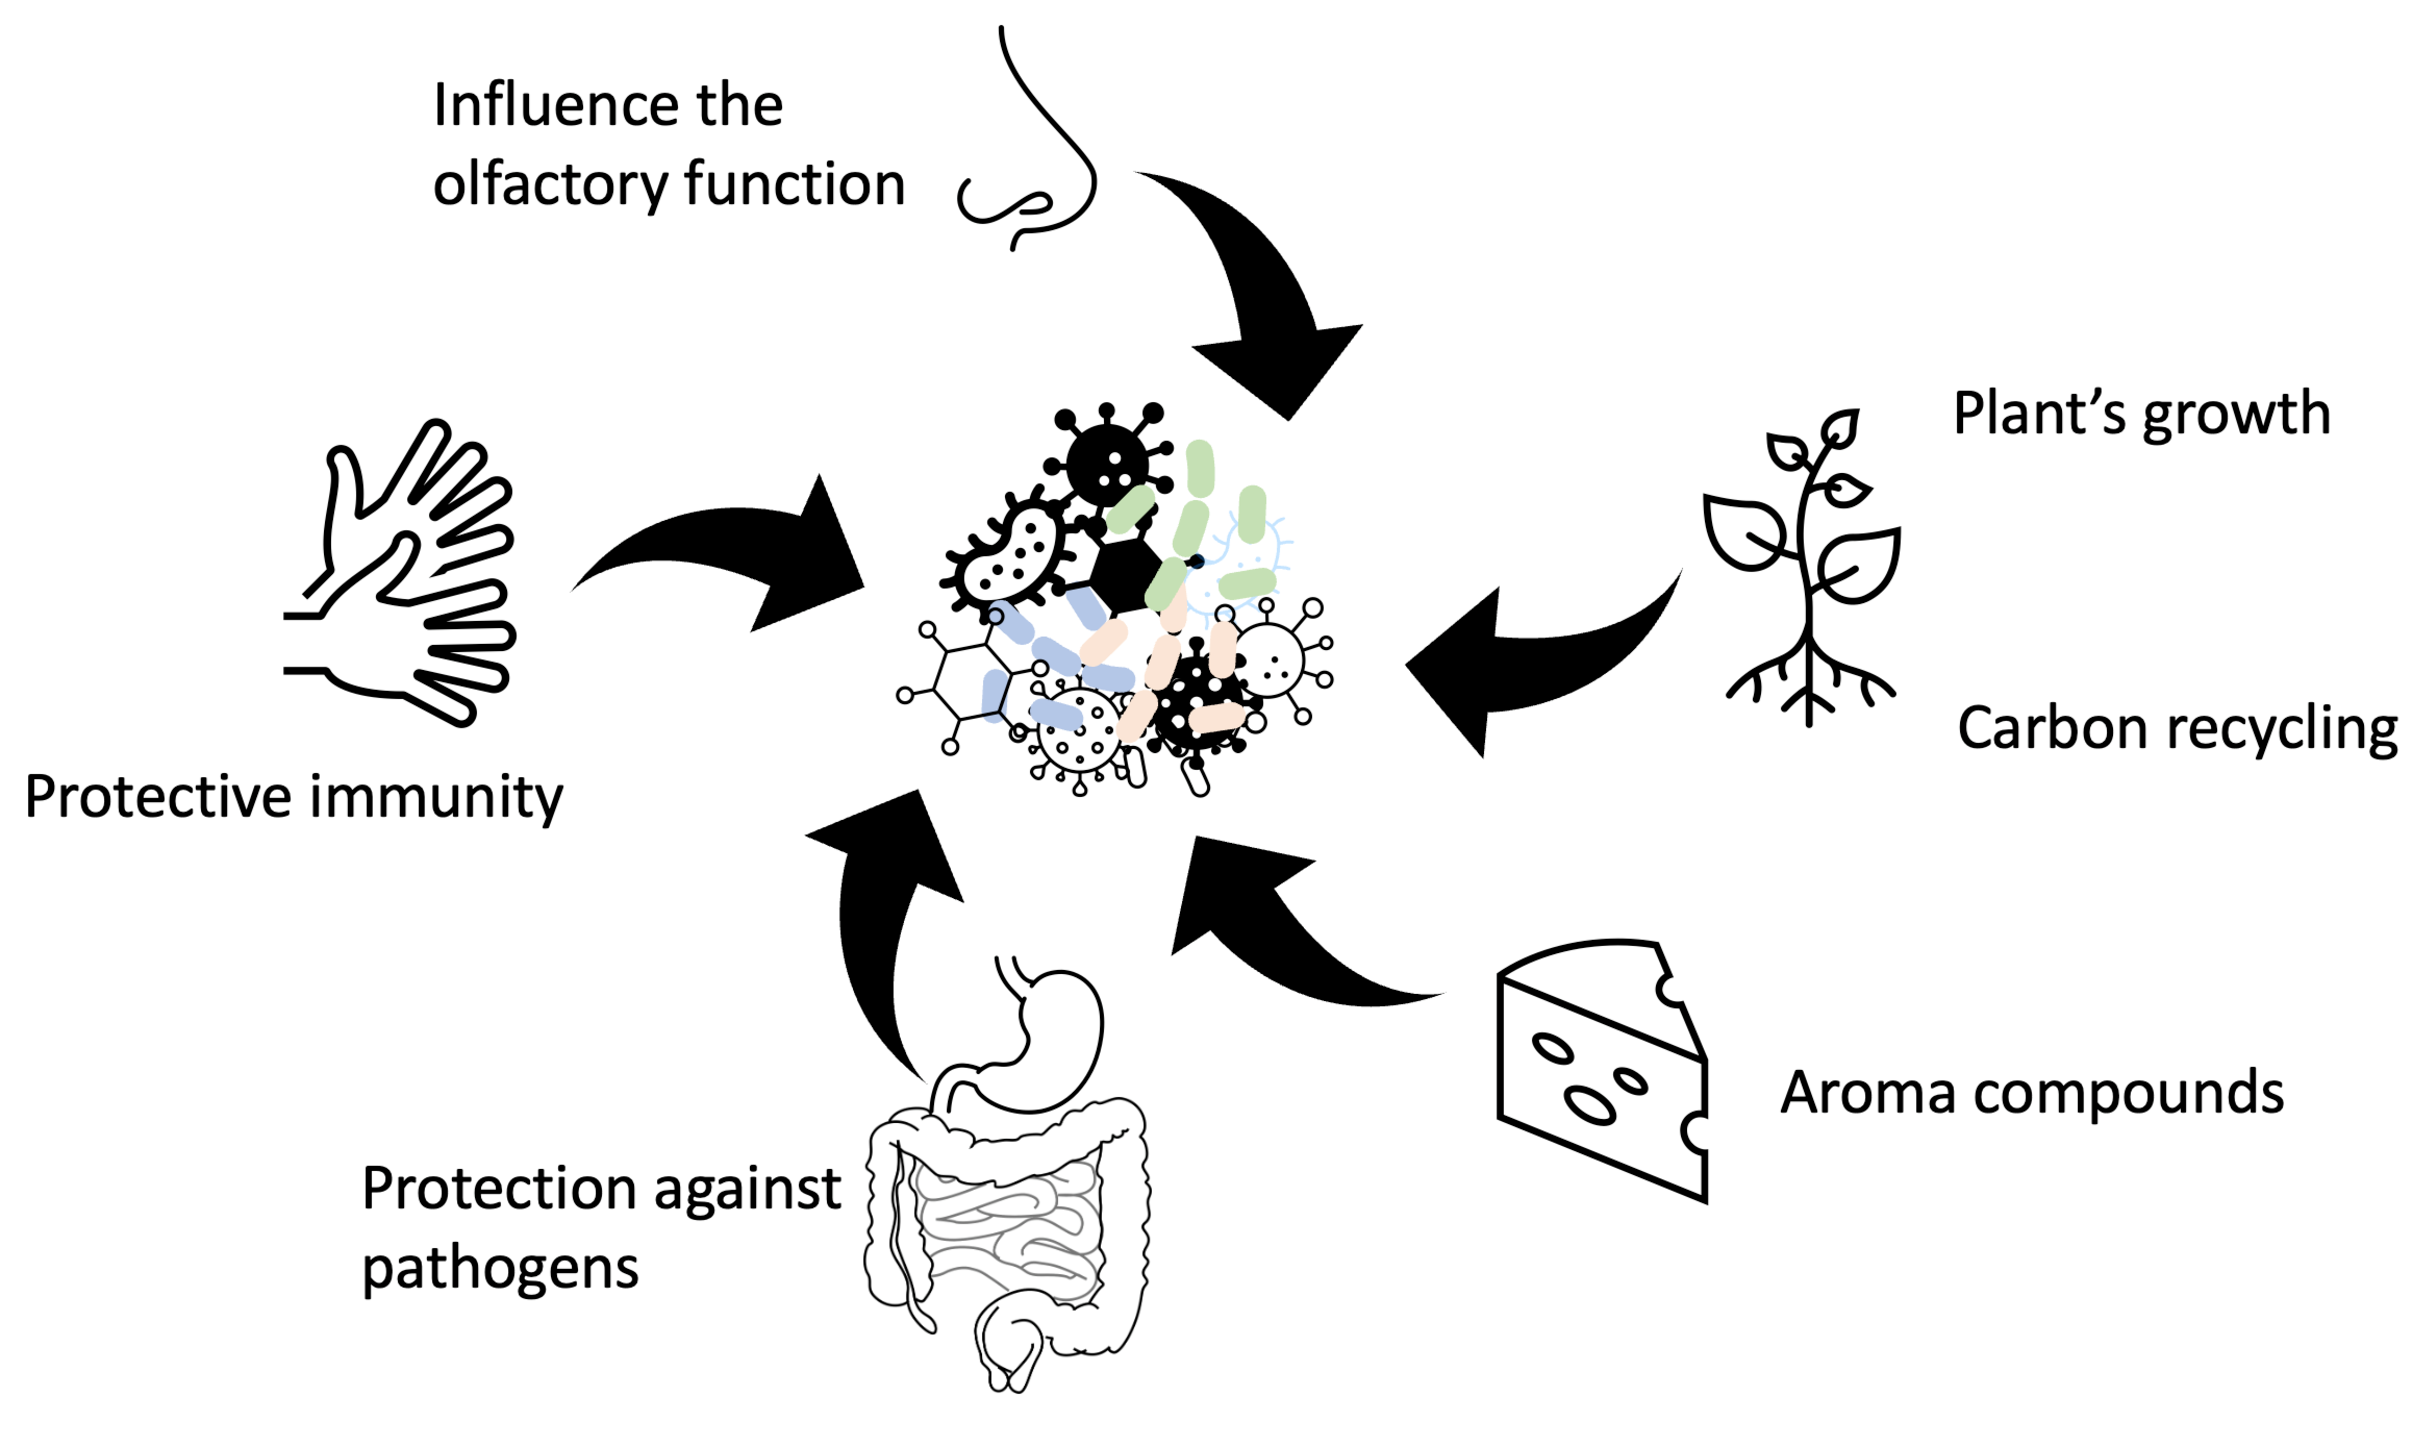
\includegraphics[width=\textwidth]{figures/bacterial-env.pdf}
\end{figure}
\end{minipage}%
\begin{minipage}{0.4\textwidth}
\textbf{In the environment}
\begin{itemize}
\item High taxonomic diversity  \\

\item High functional diversity \\

\item Complex bacterial interactions
\end{itemize}

\end{minipage}
\begin{alertblock}{}
\centering
Computational methods are required to tackle the complexity of microbial ecosystems
\end{alertblock}

 \tiny\footcite*{10.1093/chemse/bjh067,BELKAID2014121,Zhang2015,Hoorman2011,McSweeney2000}
\end{frame}

\begin{frame}
\frametitle{Bacterial interaction process}
\centering
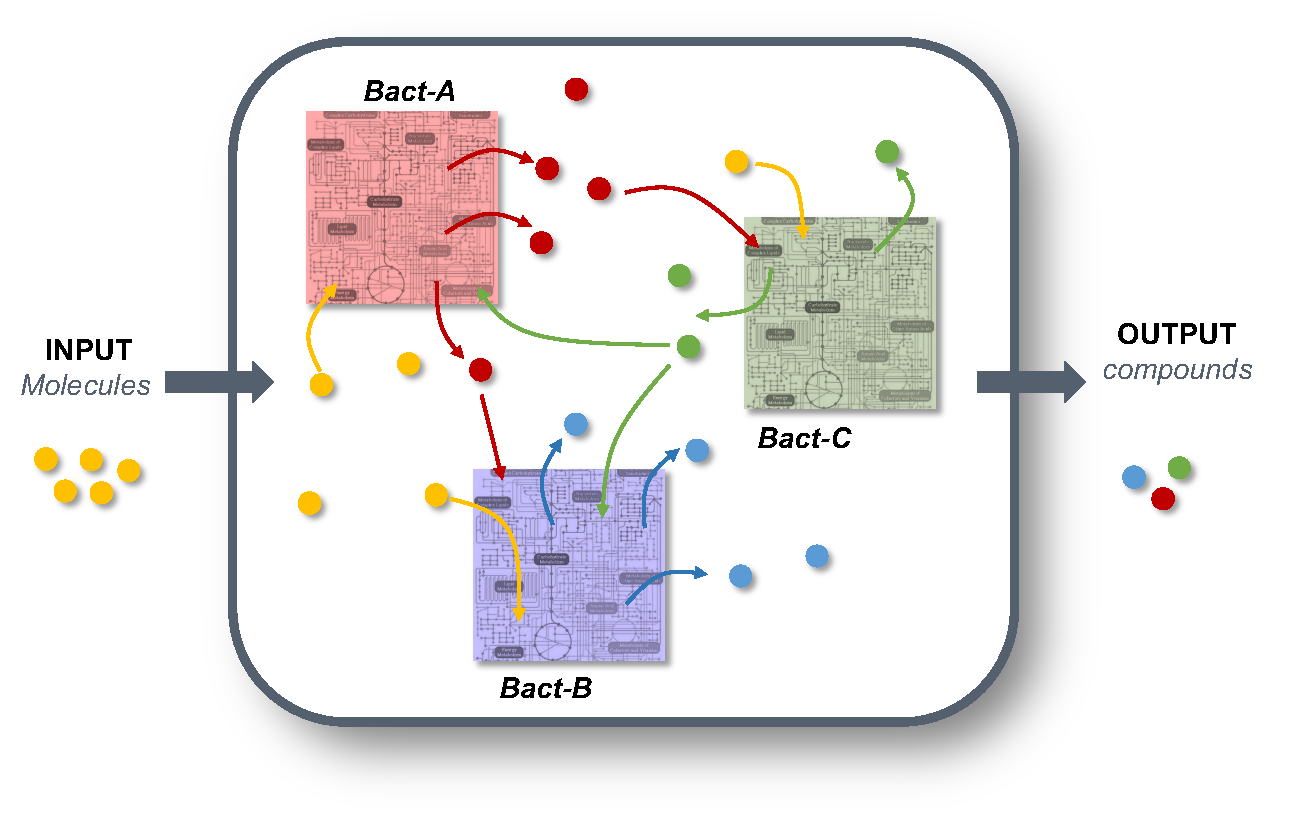
\includegraphics[width=0.9\textwidth]{figures/interactions.pdf}
\begin{itemize}
\item The direction of the exchange, species involved, ecosystem output
\end{itemize}

\begin{alertblock}{}
\centering
Mechanistic models of bacterial interactions
\end{alertblock}
\end{frame}

%\begin{frame}
%\frametitle{Hybrid approach of the metabolism}
%\textbf{The approach is hybrid}
%\begin{minipage}{0.2\textwidth}
%\begin{itemize}
%\item Temporal aspect
%\item Quantitative information
%\end{itemize}
%\end{minipage}%
%\begin{minipage}{0.6\textwidth}
%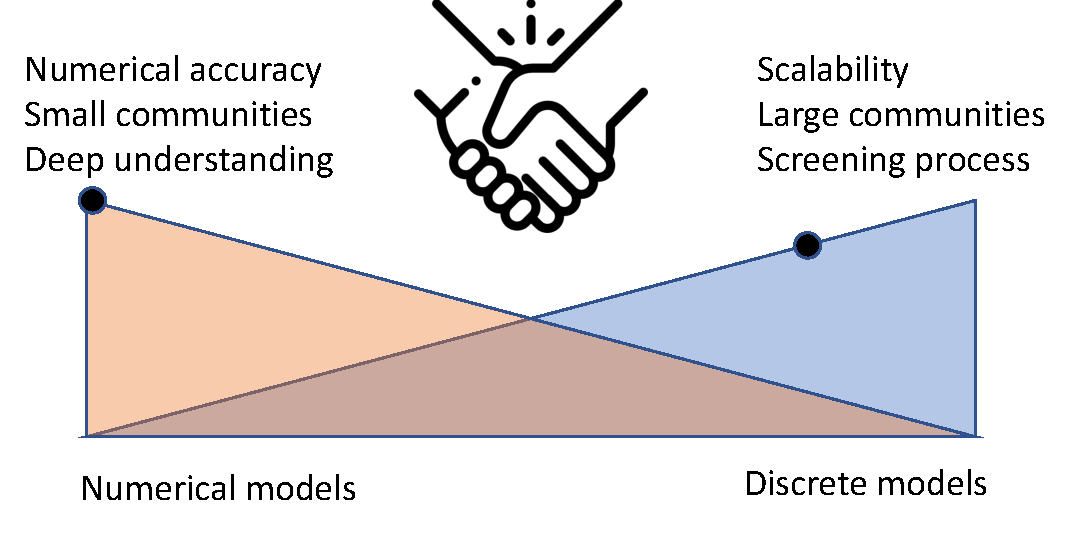
\includegraphics[width=\textwidth]{figures/further-discrete.pdf}
%\end{minipage}%
%\begin{minipage}{0.2\textwidth}
%\begin{itemize}
%\item Snapshot 
%\item Qualitative information 
%\end{itemize}
%\end{minipage}%
%
%\textbf{Hybrid background}\\
%$\rightarrow$ INRAE-Inria PhD student\\
%$\rightarrow$ Biology and computational background
%
%\begin{alertblock}{Hybrid approach}
%\centering
%Mathematical or computational formalism choice is determined from the biological issue
%%consequence: faire un choix, full numerique, discret, ou une combinaison. Ce choix est déterminé par le context d'application.
%\end{alertblock}
%\end{frame}

\begin{frame}
\frametitle{Modeling as a computational method to study microbial communities}
\begin{exampleblock}{Modeling}
Mathematical object used to simulate or predict a function
\end{exampleblock}

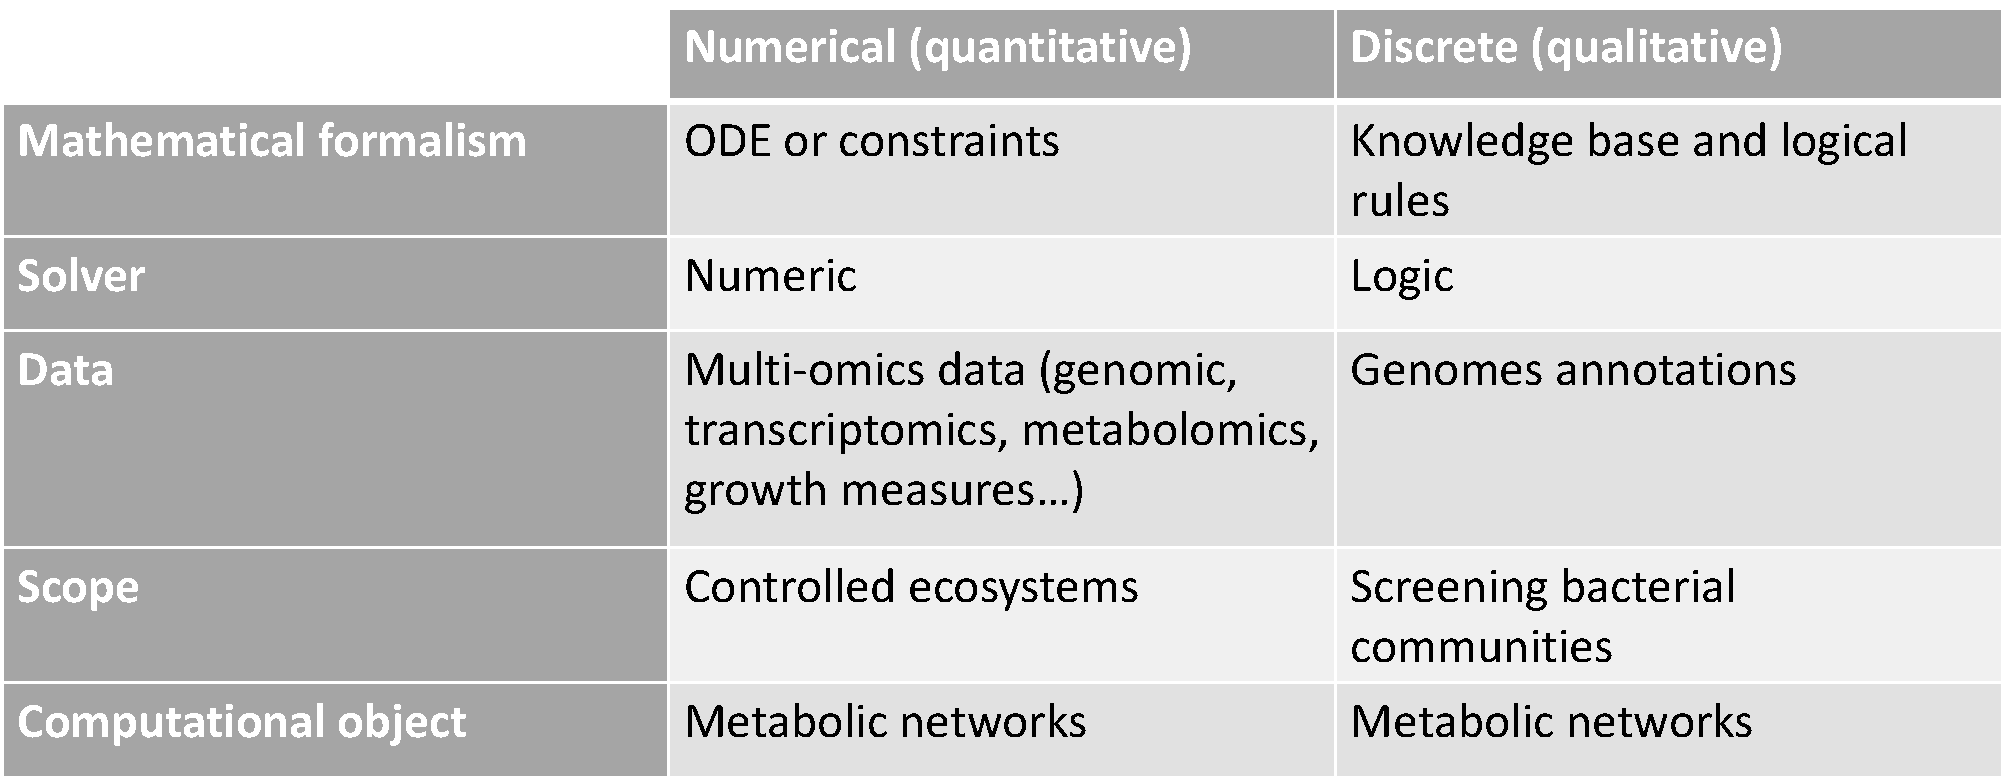
\includegraphics[width=\textwidth]{figures/modeling.pdf}

\begin{alertblock}{}
\centering
\begin{itemize}
\item Mathematical or computational formalism choice is determined by the issue
\item Metabolic modeling for understanding complex ecosystems
\end{itemize}

\end{alertblock}
\end{frame}

\begin{frame}
\frametitle{Objective and contributions}
\begin{block}{Objective}
 Contribute to analyzing metabolic interactions of bacterial communities with a hybrid approach
\end{block}

\begin{enumerate}
\item Numerical method applied to controlled community involved in cheese production $\rightarrow$ tool designed \footnote{\url{https://forgemia.inra.fr/tango/tango_models}} (\textit{in revision in Metabolic Engineering})
\begin{itemize}
\item Multi-omics data integration
\item Dynamic model $\rightarrow$ \textbf{iterative process}
\end{itemize}

\item Discrete model for screening metabolic bacterial potential in natural ecosystems $\rightarrow$ CoCoMiCo software \footnote{\url{https://gitlab.inria.fr/ccmc/CoCoMiCo}} (\textit{in prep.})

\begin{itemize}
\item Inference of \textbf{interaction properties} from KB
\end{itemize}

\item Improvement of discrete models

\begin{itemize}
\item Inference of \textbf{temporal information} from KB
\item Selection of communities based on \textbf{biological constraints} 
\end{itemize}
\end{enumerate}

\begin{alertblock}{}
\centering
Metabolic modeling for understanding complex ecosystems
\end{alertblock}

\end{frame}

\begin{frame}
\frametitle{Metabolism explains observable phenotype}
\vspace{-0.4cm}
\begin{exampleblock}{Metabolism}
Set of all biochemical reactions occurring in the cell of an organism that permit the production of energy and metabolic goods.
\end{exampleblock}
\begin{minipage}{0.5\textwidth}
$r_1 : $2 pyr $\rightarrow$ 1 aceto-Lac + 1 $\text{CO}_2$ \\
$r_2 : $1 aceto-Lac  $\rightarrow$ 1 diac  + 1 $\text{CO}_2$ \\ 
$r_3 : $1 aceto-Lac  $\rightarrow$ 1 acetoin + 1 $\text{CO}_2$ \\
$r_4 : $1 diac $\rightarrow$ 1 acetoin \\
$r_5 : $1 acetoin  $\rightarrow$1 butanediol \\

\textbf{Stoichiometry matrix}
\[
  \kbordermatrix{
     & r_1  & r_2 & r_3 & r_4 & r_5 \\
    \text{pyr}                                           & -2 & 0 & 0 & 0 & 0 \\
    \text{aceto-Lac}                      & 1 & -1 & -1 & 0 & 0  \\
    \text{diac}                      & 0 & 1 & 0 & -1 & 0  \\
    \text{CO}_2         & 1 & 1 & 1 & 0 & 0    \\
    \text{acetoin}         & 0 & 0 & 1 & 1 & -1   \\
    \text{butanediol}         & 0 & 0 & 0 & 0 & 1  \\
        }
\]

\end{minipage}%
\hspace{0.2cm}
\hfill
\begin{minipage}{0.44\textwidth}
\textbf{Bipartite graph relationship}


\begin{tikzpicture}
\node (x) [circle, draw,mystyle] at (3,8)   {pyr};
  \node (a) [circle, draw,mystyle] at (4.5,6.8)   {aceto-Lac};
    \node (b) [circle, draw,mystyle] at (4.5,4.4)   {diac};
      \node (c) [circle, draw,mystyle] at (6,6.8)   {$ \text{CO}_2 $};
        \node (d) [circle, draw,mystyle] at (4.5,3)   {acetoin};
          \node (e) [circle, draw,mystyle] at (7.5,3)   {butanediol};
          
     \node (f) [rectangle, draw] at (4.5,8) {$r_1$};
  	 \node (g) [rectangle, draw] at (4.5,5.6)  {$r_2$};
  	 \node (h) [rectangle, draw] at (6,4.4)   {$r_3$};
  	 \node (i) [rectangle, draw] at (3,4.4)   {$r_4$};
  	 \node (j) [rectangle, draw] at (6,3)   {$r_5$};

	\node () [] at (3.85,8.15) {\tiny-2};

     \graph { (x) -> (f) -> (a) };
     \graph { (x) -> (f) -> (c) };
     \graph { (a) -> (g) -> (c) };
     \graph { (a) -> (g) -> (b) };
	 \graph { (b) -> (h) -> (c) };      
	 \graph { (b) -> (h) -> (d) };            
	 \graph { (b) -> (i) -> (d) };       
	 \graph { (d) -> (j) -> (e) };                 
	 
\end{tikzpicture}
\end{minipage}

\tiny \footcite{Nava2023}
\end{frame}





%
%\begin{frame}{Contributions and objective}
%\vspace{-0.3cm}
%\begin{block}{Objective}
% Contribute to analyzing metabolic interactions of bacterial communities
%\end{block}
%\only<1>{
%\begin{figure}
%\centering
%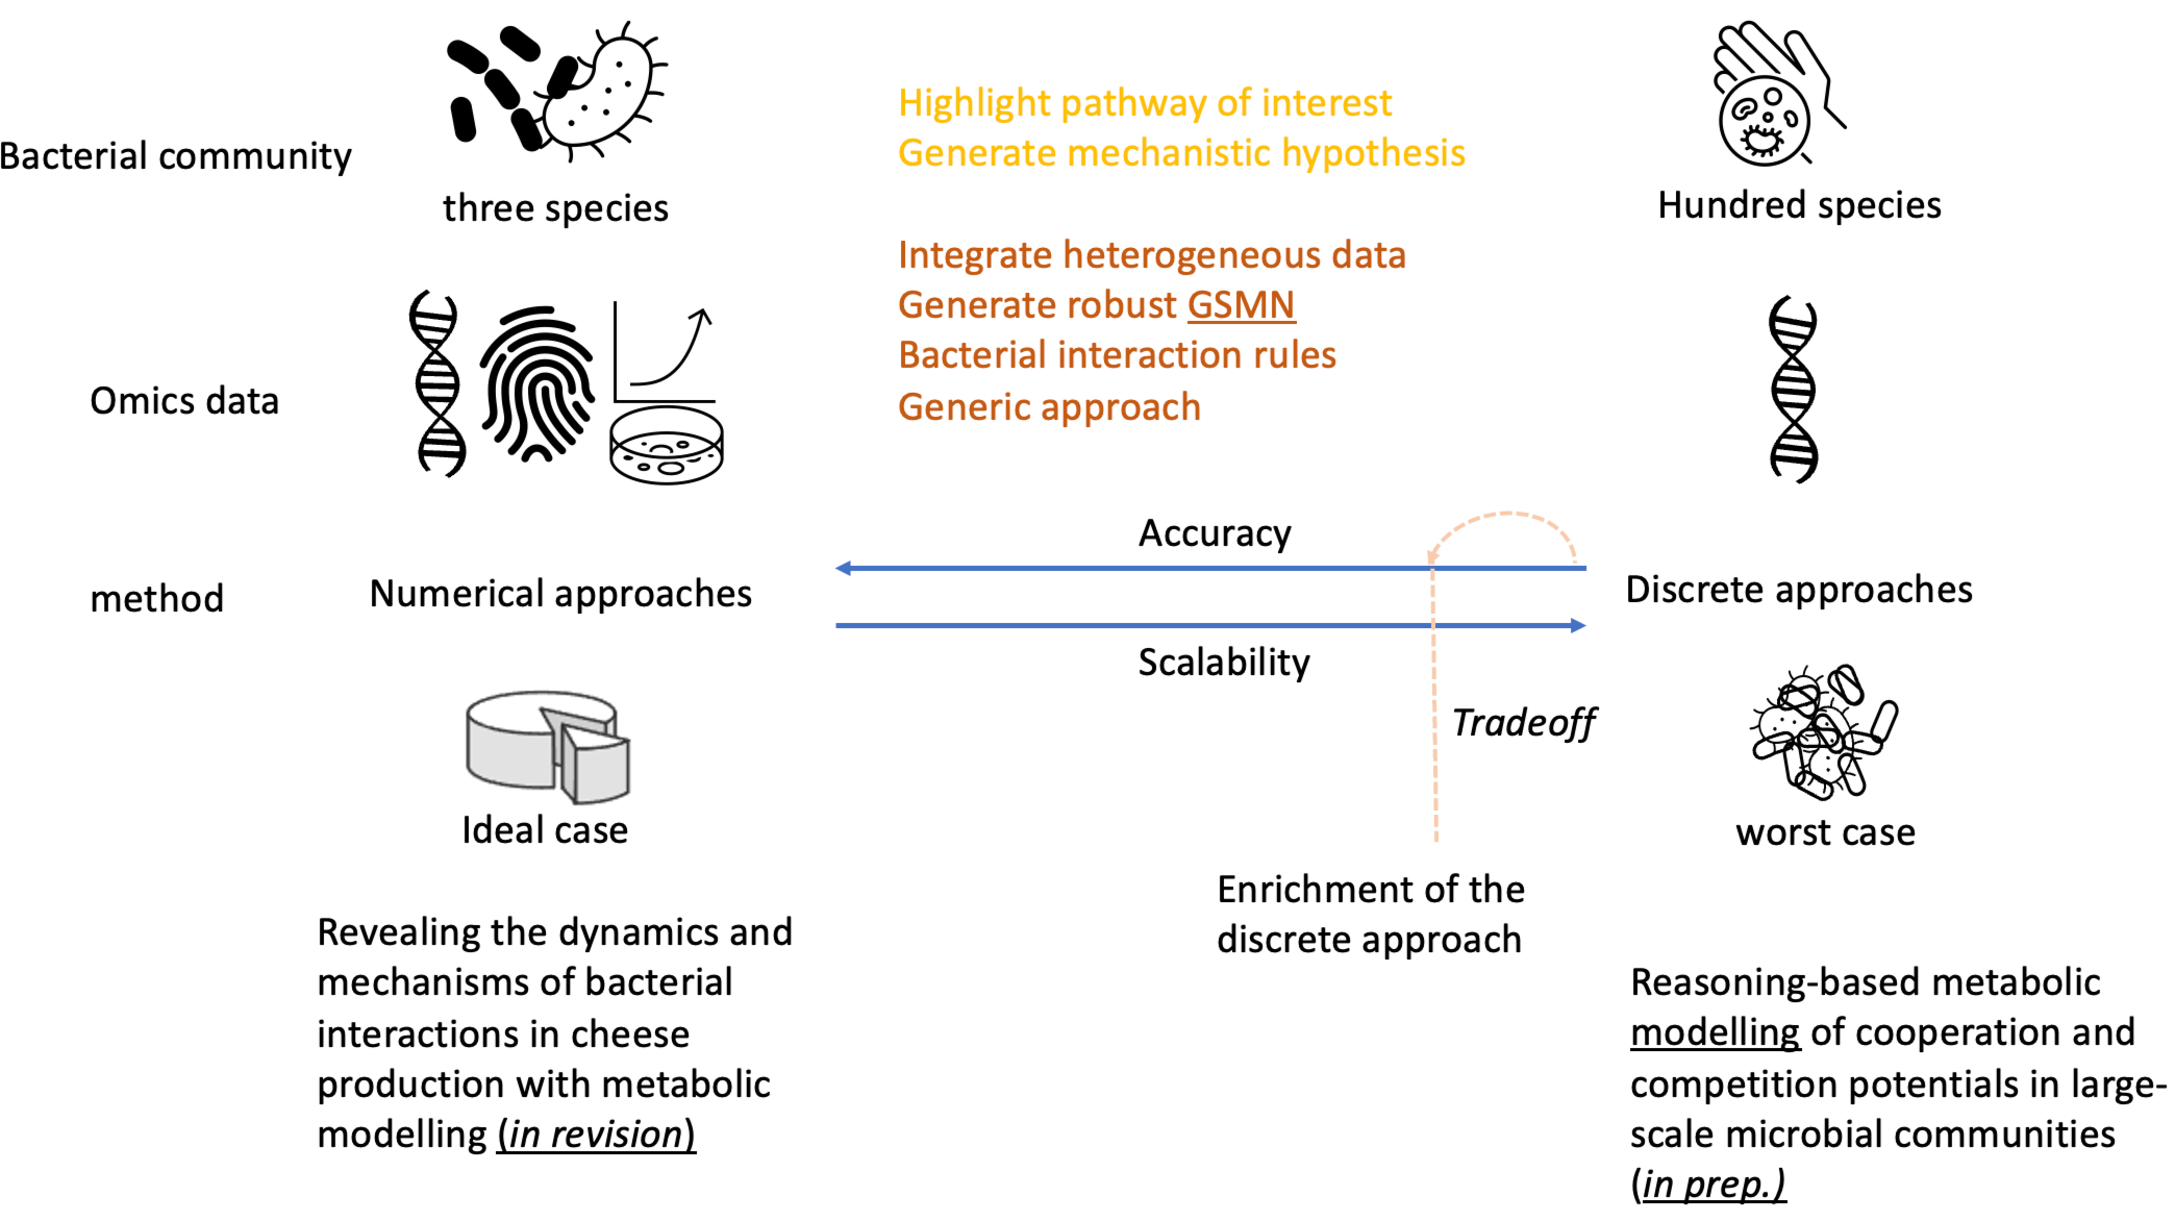
\includegraphics[width=0.8\textwidth]{figures/objective}
%\end{figure}
%\vspace{-0.5cm}
%\begin{block}{Plan}
%\begin{itemize}
%\item Dynamic and numeric model $\rightarrow$  \textbf{Iterative process} 
%\end{itemize}
%\end{block}
%}
%
%\only<2>{
%
%\begin{figure}
%\centering
%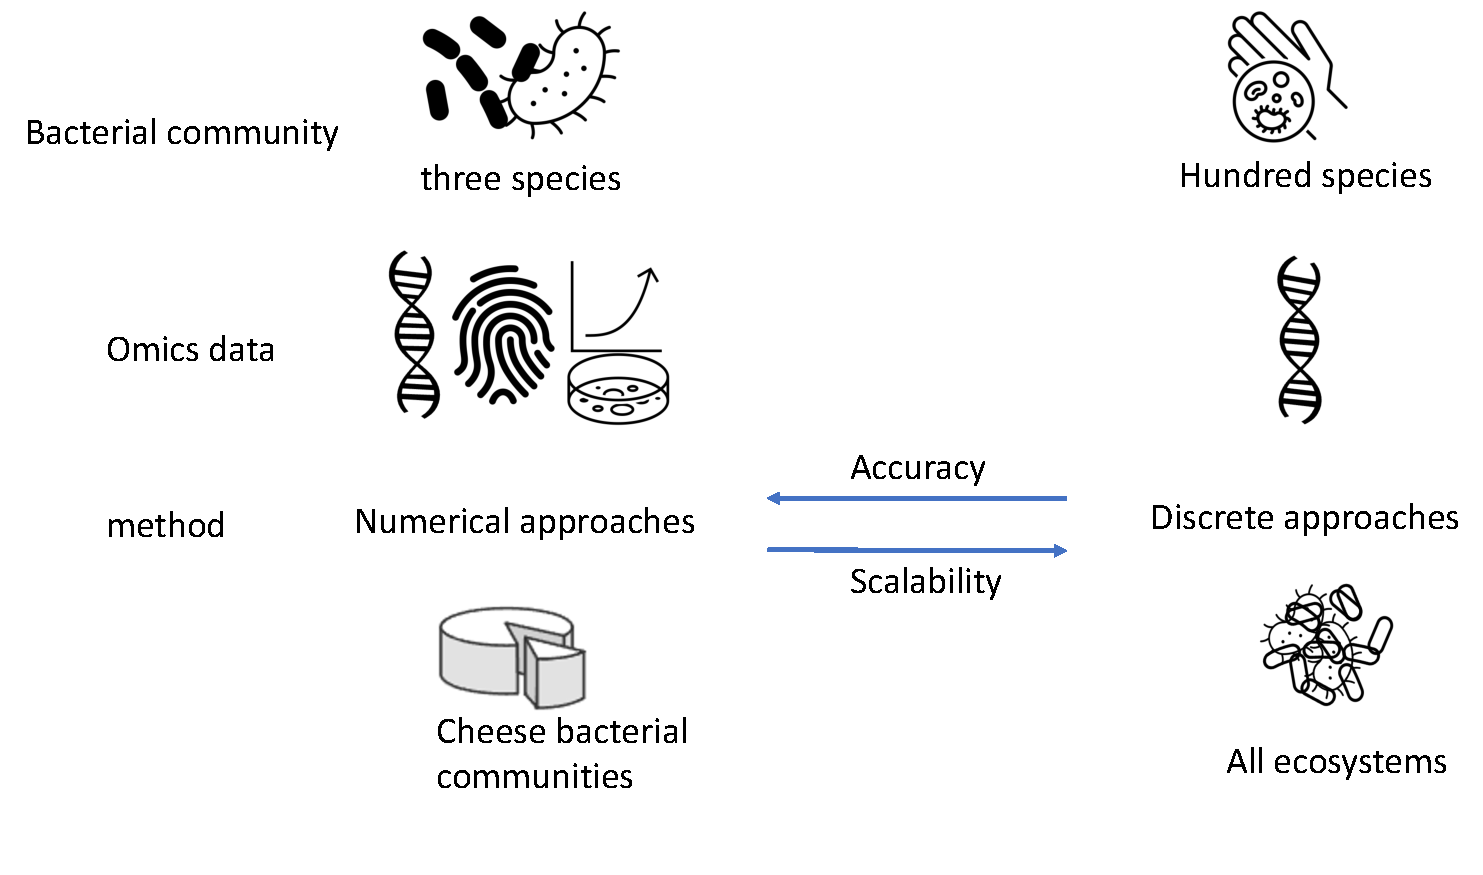
\includegraphics[width=0.8\textwidth]{figures/objective-2.pdf}
%\end{figure}
%\vspace{-0.5cm}
%\begin{block}{Plan}
%\begin{itemize}
%\item Dynamic and numeric model $\rightarrow$  \textbf{Iterative process} 
%\item Discrete model for screening potential interactions $\rightarrow$ \textbf{Interaction properties}
%\end{itemize}
%\end{block}
%
%}
%
%\only<3>{
%
%\begin{figure}
%\centering
%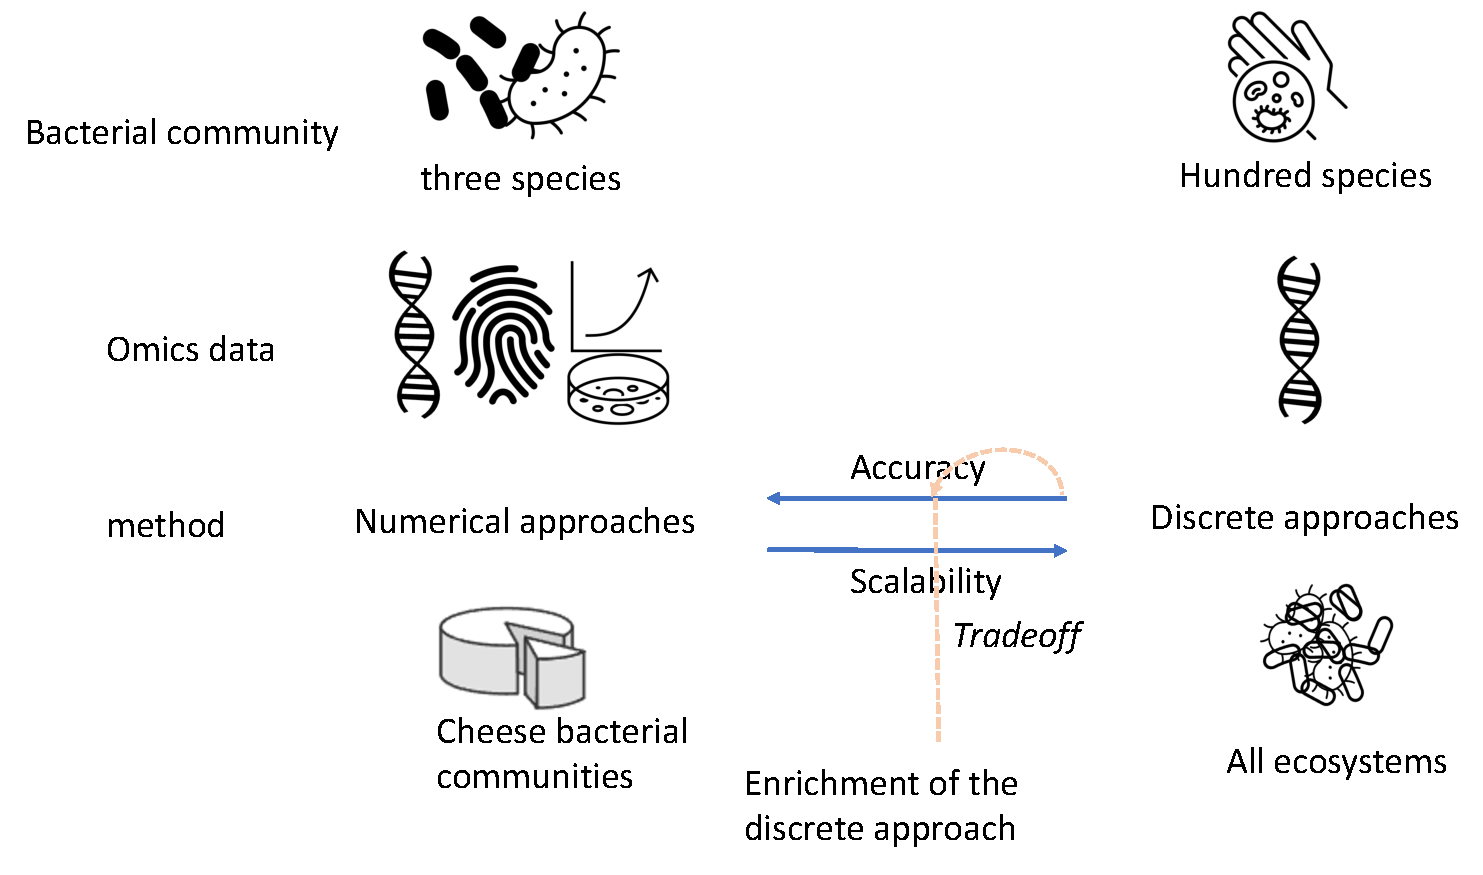
\includegraphics[width=0.8\textwidth]{figures/objective-3.pdf}
%\end{figure}
%\vspace{-0.5cm}
%\begin{block}{Plan}
%\begin{itemize}
%\item Dynamic and numeric model $\rightarrow$  \textbf{Iterative process} 
%\item Discrete model for screening potential interactions $\rightarrow$ \textbf{Interaction properties}
%\item Improvement of discrete model
%\end{itemize}
%\end{block}
%} 
%\end{frame}

\section{Numerical models}



\begin{frame}
\frametitle{Bacterial fermentation: a complex dynamic process}

\begin{figure}
\centering
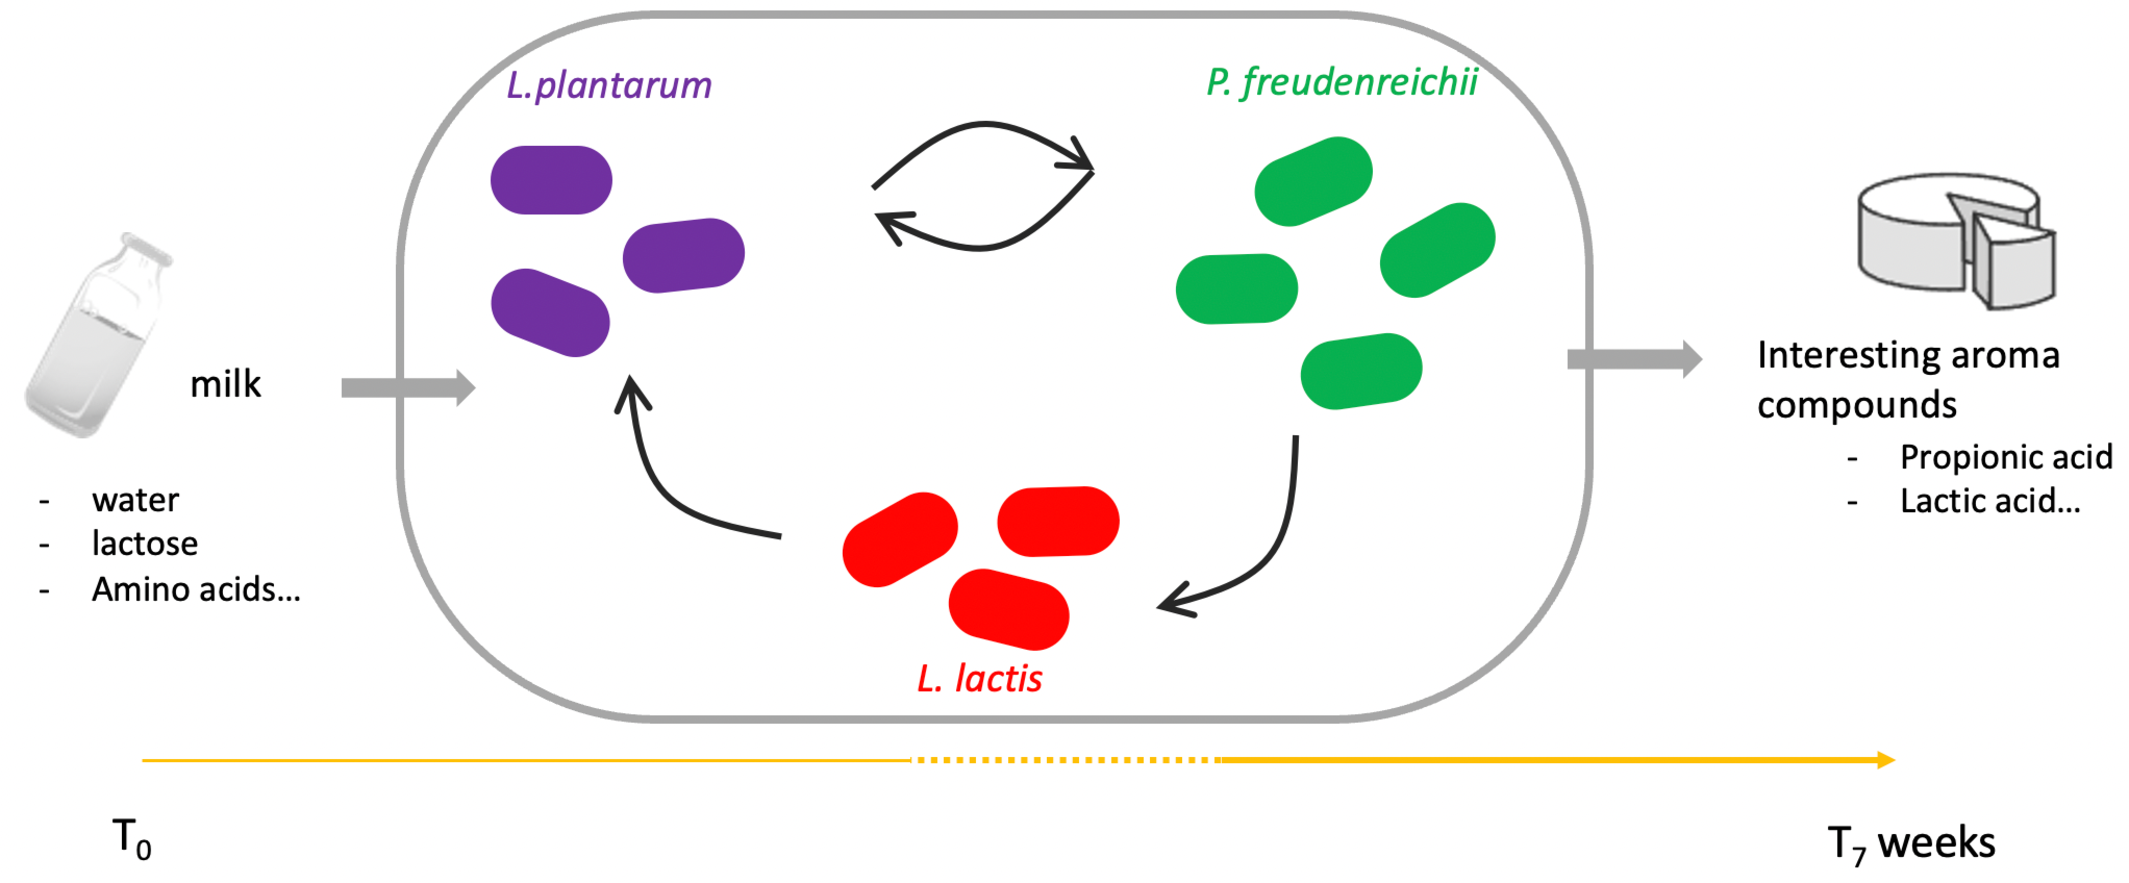
\includegraphics[width=\textwidth]{figures/context-cheese}
\end{figure}

\begin{minipage}{0.5\textwidth}
\vspace{-0.3cm}
\begin{block}{Challenge}
\begin{itemize}
\item Build coherent metabolic networks (iterative refinement) %
\item Nutrient concentration over time %
\item The dynamics of bacterial density %
\item Resource sharing between populations %
\end{itemize}
\end{block}
\end{minipage}%
\hspace{0.2cm}
\hfill
\begin{minipage}{0.45\textwidth}
\vspace{-0.55cm}
\begin{alertblock}{Solution}
\begin{itemize}
\item Create a dynamic and a numeric model of the metabolism (FBA, dFBA) 
\item TANGO implementation for characterizing bacterial interaction
\end{itemize}
\end{alertblock}
\end{minipage}

\footcite{Orth2010,Mahadevan.2002} 



\end{frame}

\begin{frame}
\frametitle{Numerical model of the metabolism -- FBA}

\only<1>{
\framesubtitle{definition}
\vspace{-3.8cm}
\begin{exampleblock}{Metabolic model}
From a GEM, a model metabolic has the capacity to simulate and to predict on the metabolic activity
\end{exampleblock}
}

\only<2>{

\framesubtitle{Flux Balance Analysis}

\begin{exampleblock}{Metabolic model}
From a GEM, a model metabolic has the capacity to simulate and to predict on the metabolic activity
\end{exampleblock}
\textbf{Constraint-based approaches}
\begin{minipage}{0.5\textwidth}

\begin{align*}
\begin{split}
    \text{maximiser/minimiser }\text{$f_{obj}$} \\
    \text{tel que } (S.v)_{int} = 0\\
    \text{et } \text{$v_{i_{min}}$} \leq v_i \leq \text{$v_{i_{max}}$}
\end{split}
\end{align*}

\begin{figure}
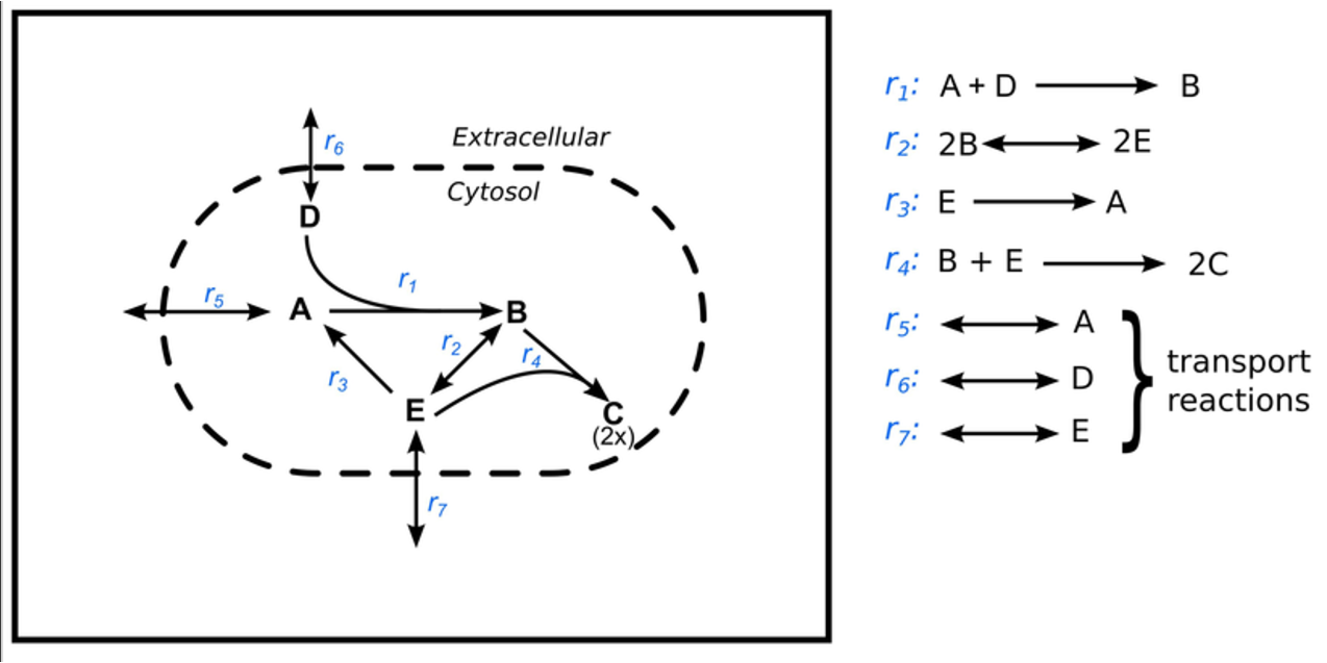
\includegraphics[width=\textwidth]{figures/mass-balance-1}
\vspace{-0.5cm}\caption{Example of a metabolic network}
\end{figure}

\end{minipage}%
\begin{minipage}{0.5\textwidth}
\begin{figure}
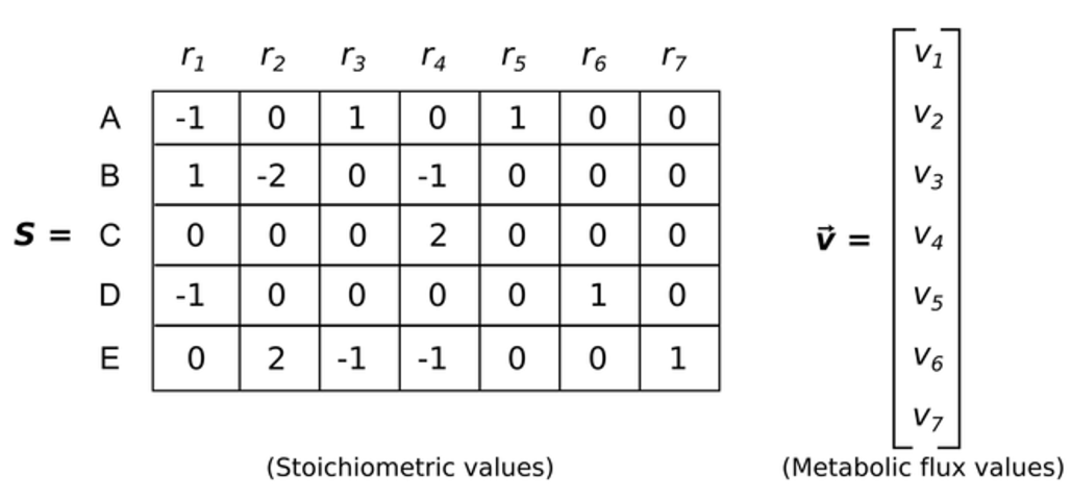
\includegraphics[width=\textwidth]{figures/mass-balance-2}
\caption{A. Stoichiometry matrix representation and the flux vector v}
\end{figure}

\end{minipage}

}

\only<3> {

\framesubtitle{Flux Balance Analysis}

\begin{exampleblock}{Metabolic model}
From a GEM, a model metabolic has the capacity to simulate and to predict on the metabolic content
\end{exampleblock}
\textbf{Constraint-based approaches}
\begin{minipage}{0.5\textwidth}

\begin{align*}
\begin{split}
    \text{maximiser/minimiser }\text{$f_{obj}$} \\
    \text{tel que } (S.v)_{int} = 0\\
    \text{et } \text{$v_{i_{min}}$} \leq v_i \leq \text{$v_{i_{max}}$}
\end{split}
\end{align*}

\begin{figure}
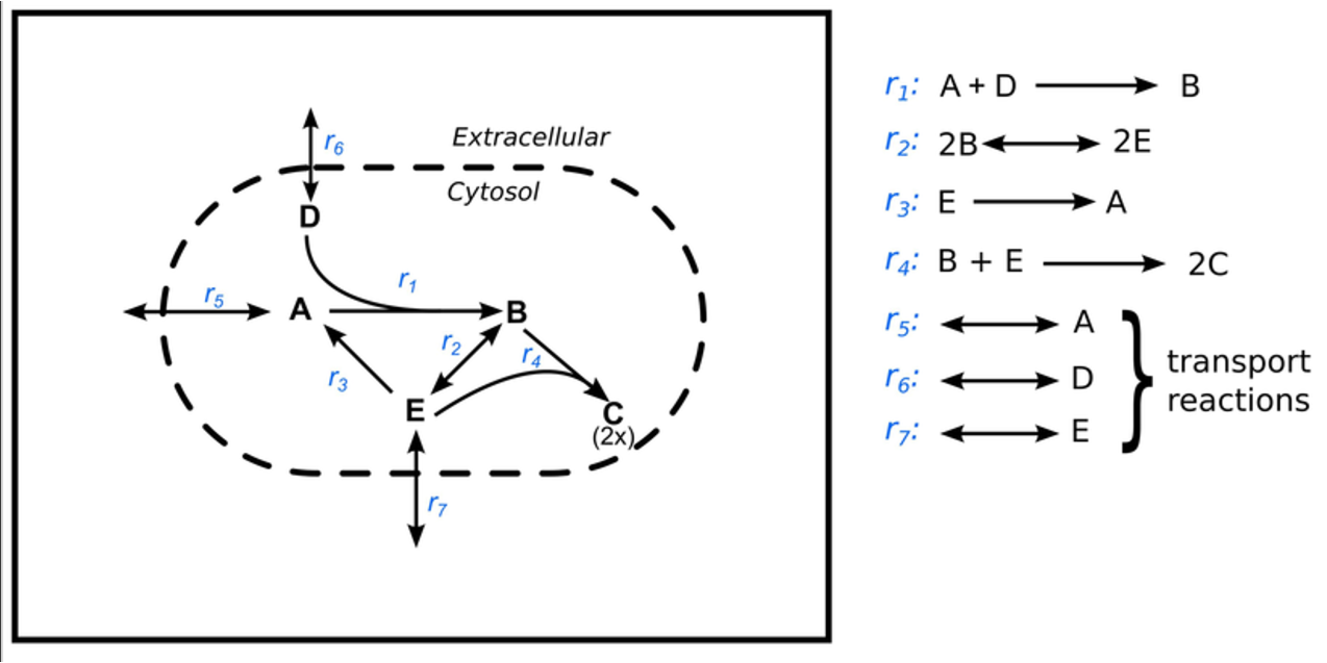
\includegraphics[width=\textwidth]{figures/mass-balance-1}
\vspace{-0.5cm}\caption{Example of a metabolic network}
\end{figure}

\end{minipage}%
\begin{minipage}{0.5\textwidth}
\begin{figure}
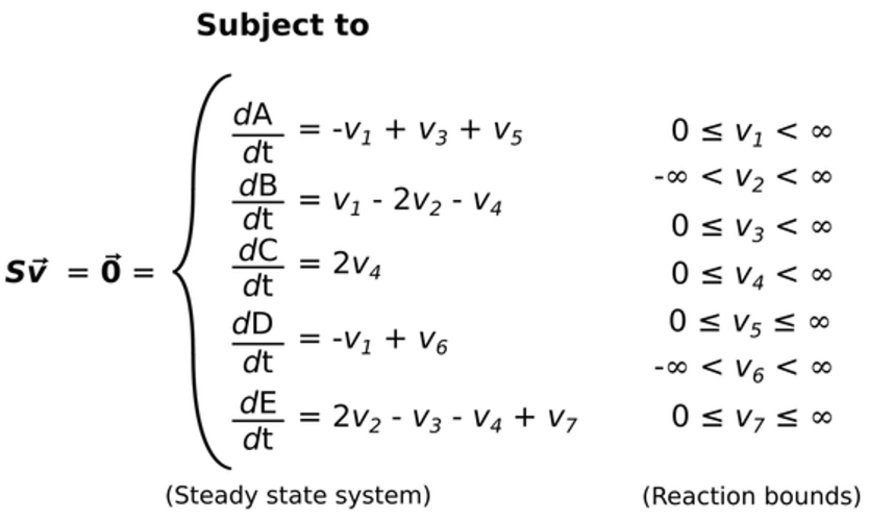
\includegraphics[width=\textwidth]{figures/mass-balance-3}
\caption{B. Linear programming problem.}
\end{figure}

\end{minipage}

}

\footcite{Orth2010}

\end{frame}

\begin{frame}
\frametitle{FBA genome-scale metabolic model refinement}
\begin{itemize}
\item Modify reactions (flux, add, remove)
\item Verify known pathway and metabolic activities
\end{itemize}

\only<1>{
\begin{figure}
\begin{minipage}{0.5\textwidth}
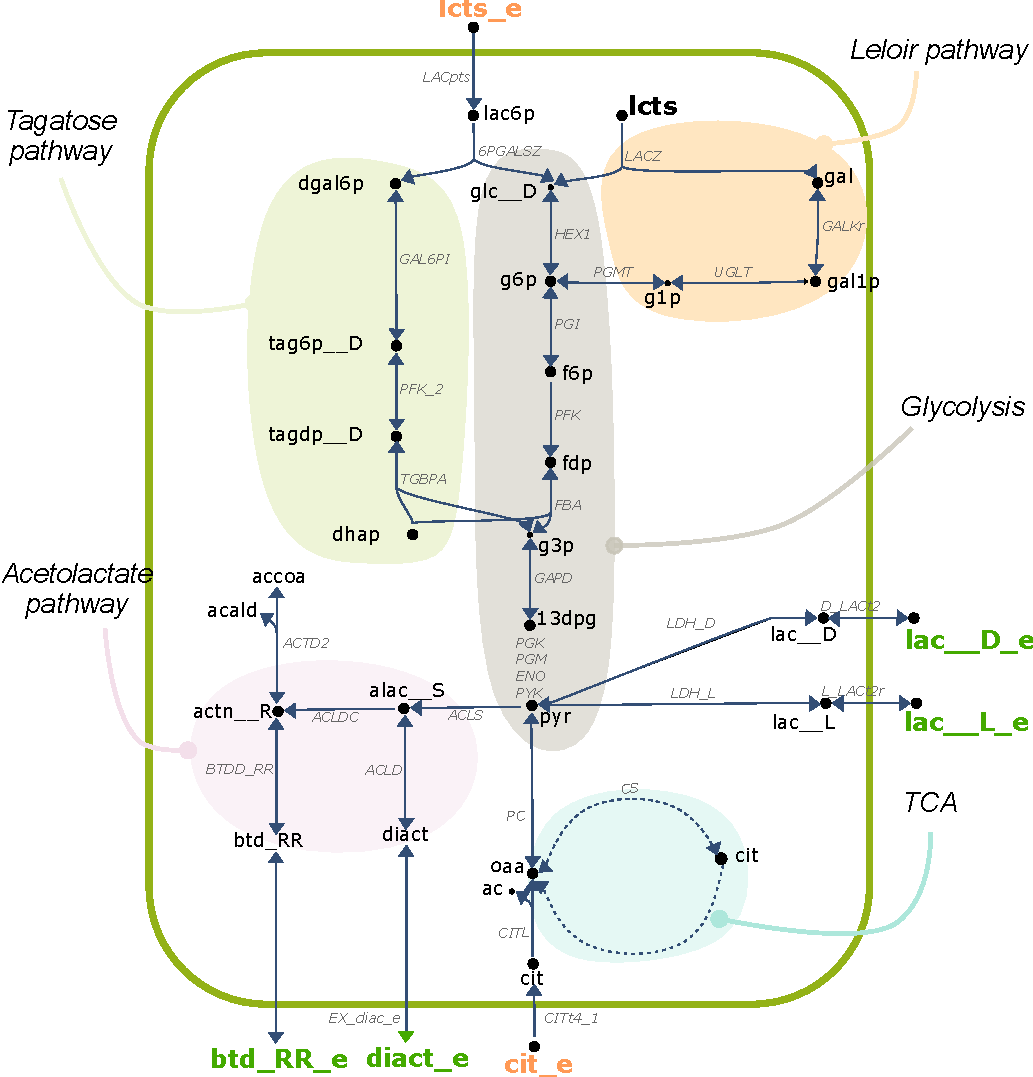
\includegraphics[width=0.9\textwidth]{figures/carte_lactis.pdf}\\
Initial metabolic map
\end{minipage}%
\hspace{0.4cm}
\hfill
\begin{minipage}{0.4\textwidth}
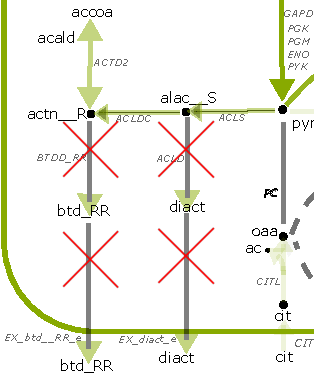
\includegraphics[width=0.8\textwidth]{figures/FIG2_opt_explo_ll_before.pdf}\\
FBA show missing expected activities
\end{minipage}

\end{figure}


}

\only<2>{
\begin{figure}
\begin{minipage}{0.5\textwidth}
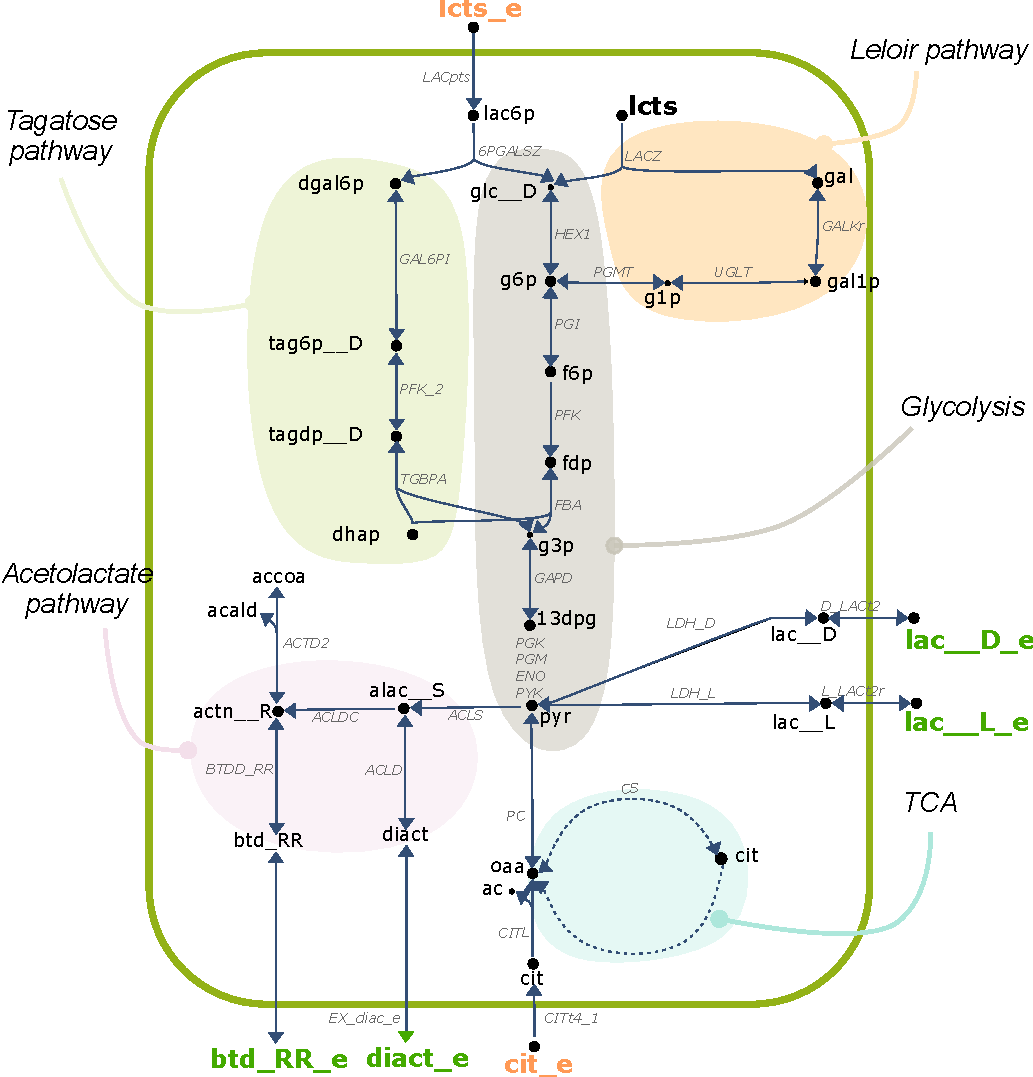
\includegraphics[width=0.9\textwidth]{figures/carte_lactis.pdf}\\
Initial metabolic map
\end{minipage}%
\hspace{0.4cm}
\hfill
\begin{minipage}{0.4\textwidth}
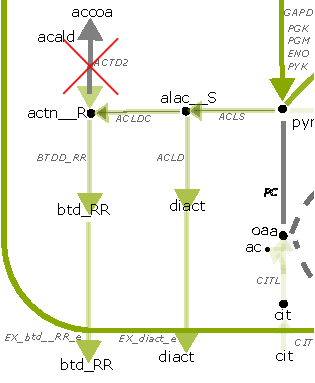
\includegraphics[width=0.8\textwidth]{figures/FIG2_opt_explo_ll_after.pdf}\\
Constraining ACTD2 reaction
\end{minipage}

\end{figure}

\begin{alertblock}{Improvement}
Modification reaction bounds in the model and in the software
\end{alertblock}
}

\footcite{Carroll1999,Swindell1996,Makhlouf2006}

\end{frame}

\begin{frame}
\frametitle{Dynamic model of the metabolism}
\begin{exampleblock}{dFBA}
\begin{itemize}
\item FBA at each time point
\item Previous time point output used as input for the next time point
\end{itemize}
\end{exampleblock}
\textbf{FBA}
\begin{align*}
F_j & =\sum_{i \in \mathcal{B}} {\mu}_{i,j}\left((c^{ex}_{min,i},c^{ex}_{max,i})(b^n,m^n)\right) b_i \\
\end{align*}
\vspace{-1cm}
\begin{figure}[t]
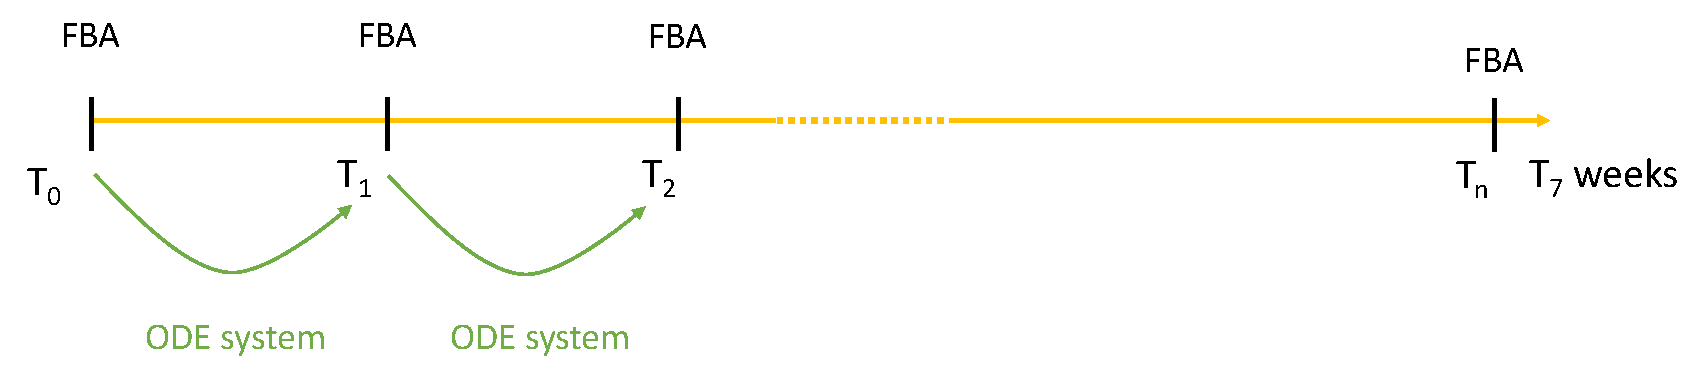
\includegraphics[width=\textwidth]{figures/time-dfba.pdf}
\end{figure}
\vspace{-0.3cm}
\textbf{ODE System}
\begin{align*}
b_i^{n+1}& = b_i^n+\Delta t* F_{b_i} \\
m_j^{n+1}& =\begin{cases} m_i^n+\Delta t* F_{j} & \text{ si } F_j>0 \\ %\text{ (cas explicite)}\\
m_j^n/(1-\Delta t * F_j/m_j^n) & \text{ sinon} \\ % (cas implicite)}
\end{cases}
\end{align*}
\footcite{Mahadevan.2002}
\end{frame}

\begin{frame}
\frametitle{Parameter inference}
\begin{block}{}
\begin{itemize}
\item Make individual GSMN accurate for inferring mechanistic bacterial behavior
\item Finding optimal parameters for explaining \textbf{species level} biological observations
\item Quantitative check of metabolic goods and biomass density
\end{itemize}
\end{block}
\only<1>{
\textbf{Lactic Acid Bacteria (LAB)} 

\begin{equation}
J(b_i,pH | \theta_i, b_{i,exp},pH_{exp} ) = \left \Vert \frac{\logten(b_i) - \logten(b_{i,exp})}{\sigma_{log,i,exp}} \right \Vert^2 + \alpha \left \Vert\frac{pH - pH_{exp}}{\sigma_{pH,exp}} \right \Vert^2 
\label{eq:optim_LAB}
\end{equation}

\begin{minipage}{0.5\textwidth}
\begin{figure}
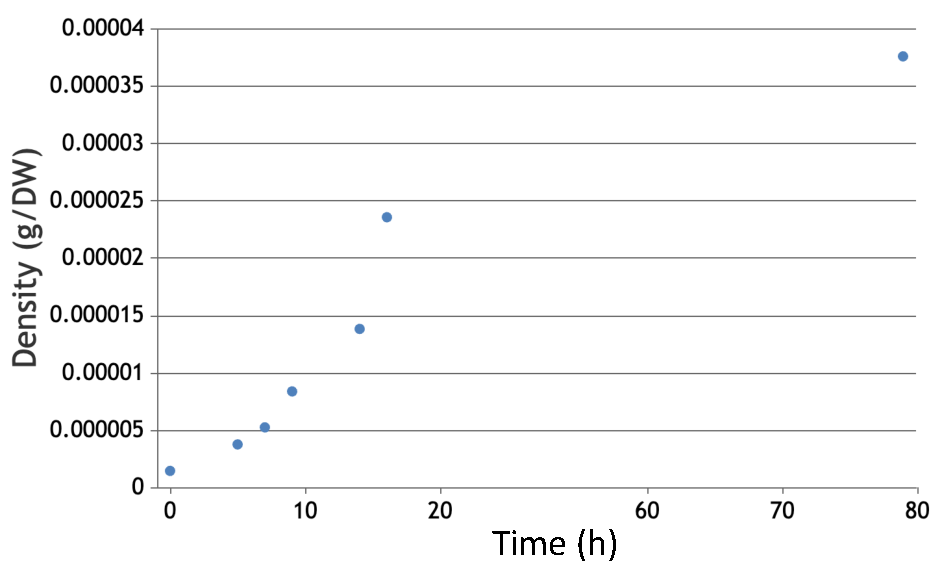
\includegraphics[width=0.8\textwidth]{figures/ind-data-plantarum.pdf}
\end{figure}
\end{minipage}%
\begin{minipage}{0.5\textwidth}
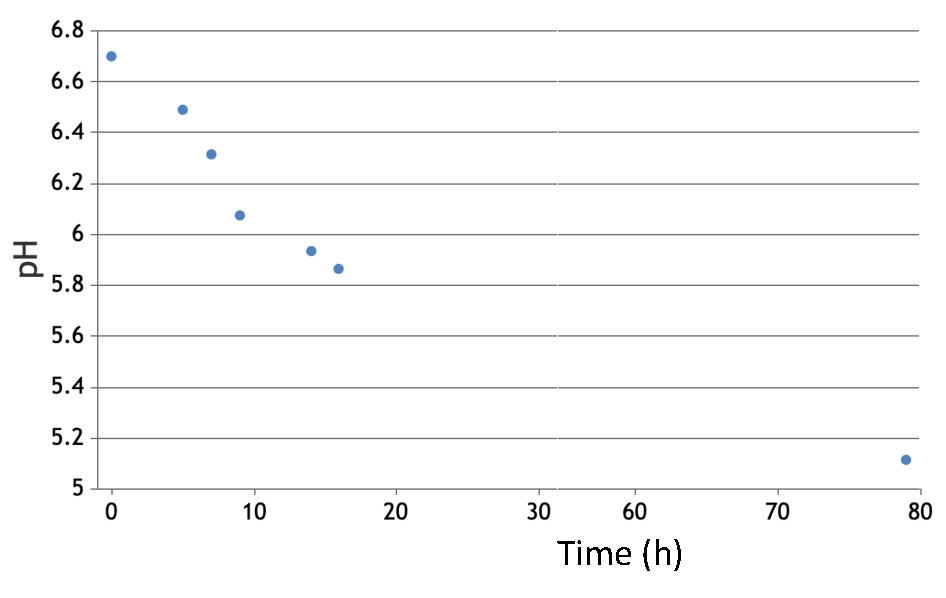
\includegraphics[width=0.8\textwidth]{figures/ph-data-lactis.pdf}
\end{minipage}%

\begin{block}{Environmental condition}
\begin{itemize}
\item Milk
\end{itemize}
\end{block}
}

\only<2>{

\textbf{\textit{P. freudenreichii}}

\begin{equation} 
J(b,m | \theta_i, b_{exp},m_{exp} ) = \left \Vert \frac{\logten(b) - \logten(b_{exp})}{\sigma_{log,b,exp}} \right \Vert ^2 + \alpha \left \Vert \frac{m - m_{exp}}{\sigma_{m,exp}} \right \Vert^2 
\label{eq:optim_freud}
\end{equation}
\begin{table}[H]
\centering
\begin{adjustbox}{width=0.9\textwidth}
\begin{tabular}{|c|c|c|c|}
\hline
Acids & Concentration $T_0$ & Concentration $T_{f}$ = 89 h  & Standard error \\
\hline
Lactate & 16.5 & 7.88 & 0.08 \\
Acetate & 0 & 3.07 & 0.02\\
Succinate & 0 & 0.371 & 0.063 \\
Propionate & 0 & 8.31 & 0.02 \\
 \hline
\end{tabular}
\end{adjustbox}
\caption{Acids concentrations data in g/L}
\label{table:acids-dosage}
\end{table}

\begin{block}{Environmental condition}
\begin{itemize}
\item Milk + lactate + peptone
\end{itemize}
\end{block}


}
\end{frame}

\begin{frame}
\frametitle{Dynamic control of the metabolism}

\textbf{Defining consumption limitation in the model}

\begin{equation}
c^{ex}_{min,i,j} = max(-\frac{m_{j}}{\Delta t*\sum_{i \in \mathcal{M_j}} b_i}, v^{int}_{i,j})
\end{equation}


\begin{itemize}
\item $\mathcal{M_j}$ Bacteria subset can metabolize $_j$
\item $v^{int}_{i,j}$ close to the FBA value
\item Balanced resource sharing \\
\end{itemize}
\vspace{1cm}
\textbf{Lactose consumption case for LAB}

1- Calculation of pH  from lactate concentration\\

\[
pH = pKa_{lac} c_1 * (m_{lac\_\_L\_e}+m_{lac\_\_D\_e})+c_2
\]


2- Regulation of lactose consumption \\
\begin{equation}
c^{ex}_{min,i,j} = max(-\frac{m_{lcts_e}}{\Delta t*\sum_{i \in \mathcal{M}(lcts_e)} b_i},-\mu_{max,lcts}*10^{(-k_{lac}*\phi_{undiss})}-\mu_{min,lcts})
\end{equation}

\footcite{Ozcan.2020}

\end{frame}

\begin{frame}
\frametitle{Individual model validation}
\begin{minipage}{0.5\textwidth}
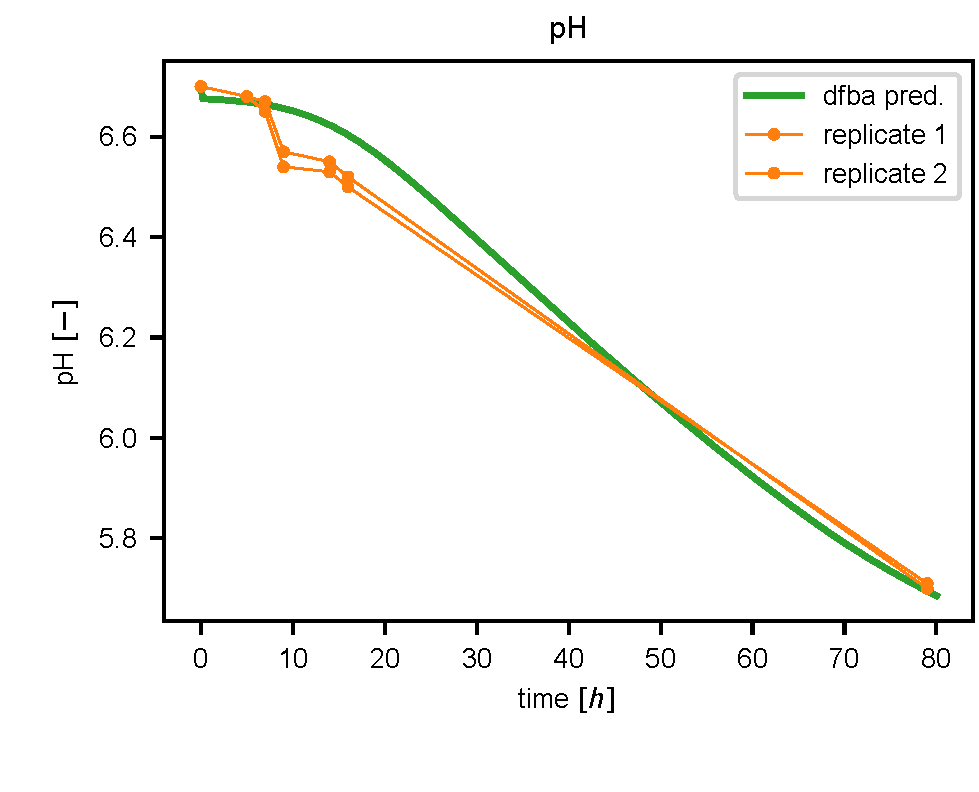
\includegraphics[width=\textwidth]{figures/validation-lp.pdf}
\end{minipage}%
\begin{minipage}{0.5\textwidth}
\vspace{-0.5cm}
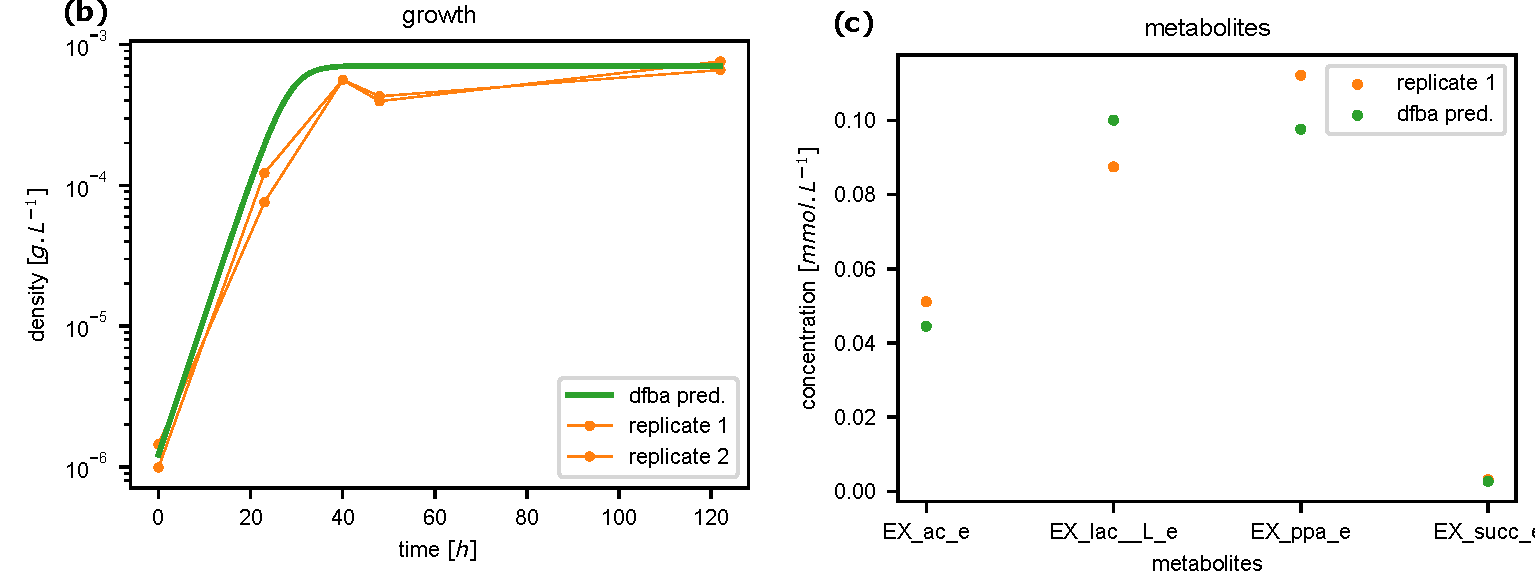
\includegraphics[width=\textwidth]{figures/validation-pf.pdf}
\end{minipage}
\begin{minipage}{0.5\textwidth}
\vspace{-0.3cm}
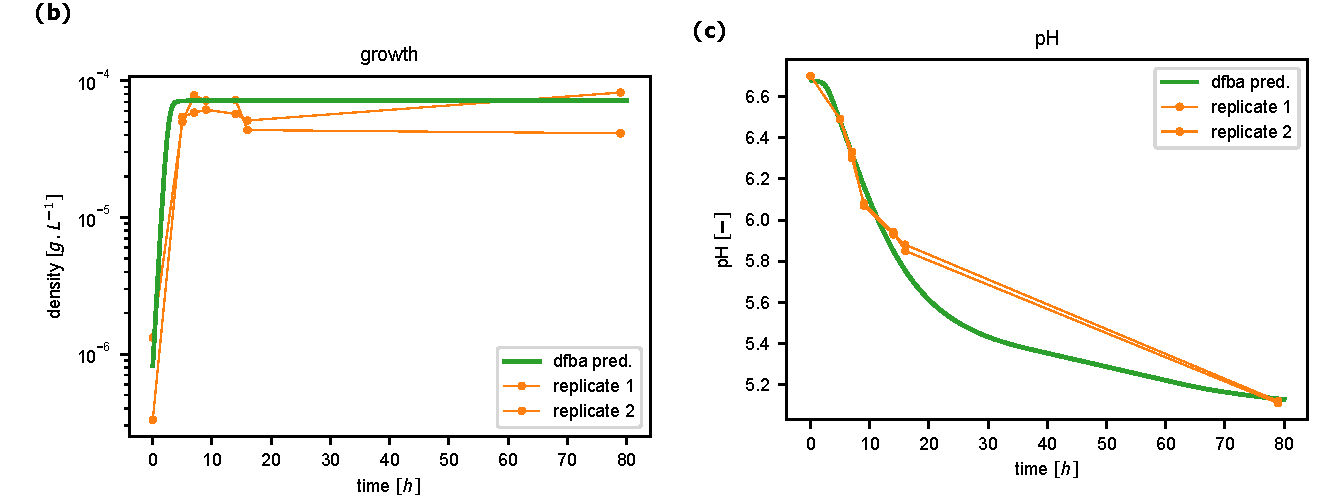
\includegraphics[width=\textwidth]{figures/validation-ll.pdf}
\end{minipage}%
\hspace{0.3cm}
\hfill
\begin{minipage}{0.4\textwidth}
\begin{block}{Results after parameters inference}
Individual metabolic models are well calibrated $\rightarrow$ reproduce experimental data
\end{block}

\end{minipage}

\end{frame}

\begin{frame}
\frametitle{Community validation}

\begin{figure}
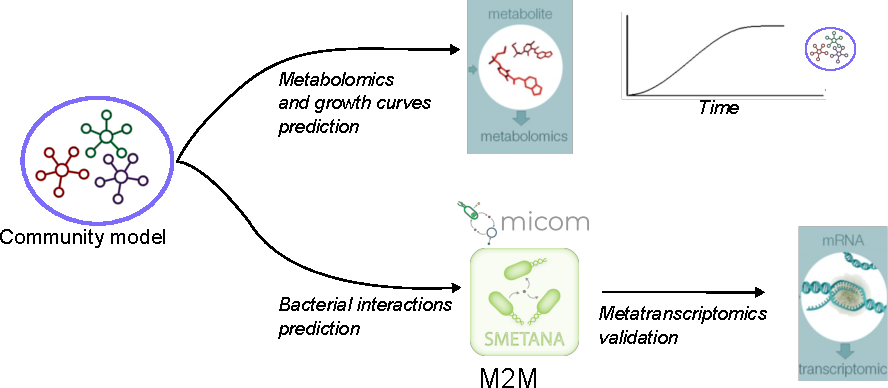
\includegraphics[width=\textwidth]{figures/com-validation.pdf}
\end{figure}
\begin{block}{}
\begin{itemize}
\item Bacterial interaction \textbf{prediction}
\item Metabolic explanation of biological observations
\item \textbf{No community calibration}
\end{itemize}
\end{block}
\footcite{Cao2021}

\end{frame}

\begin{frame}
\frametitle{Community prediction}
\framesubtitle{Growth and pH}
\centering
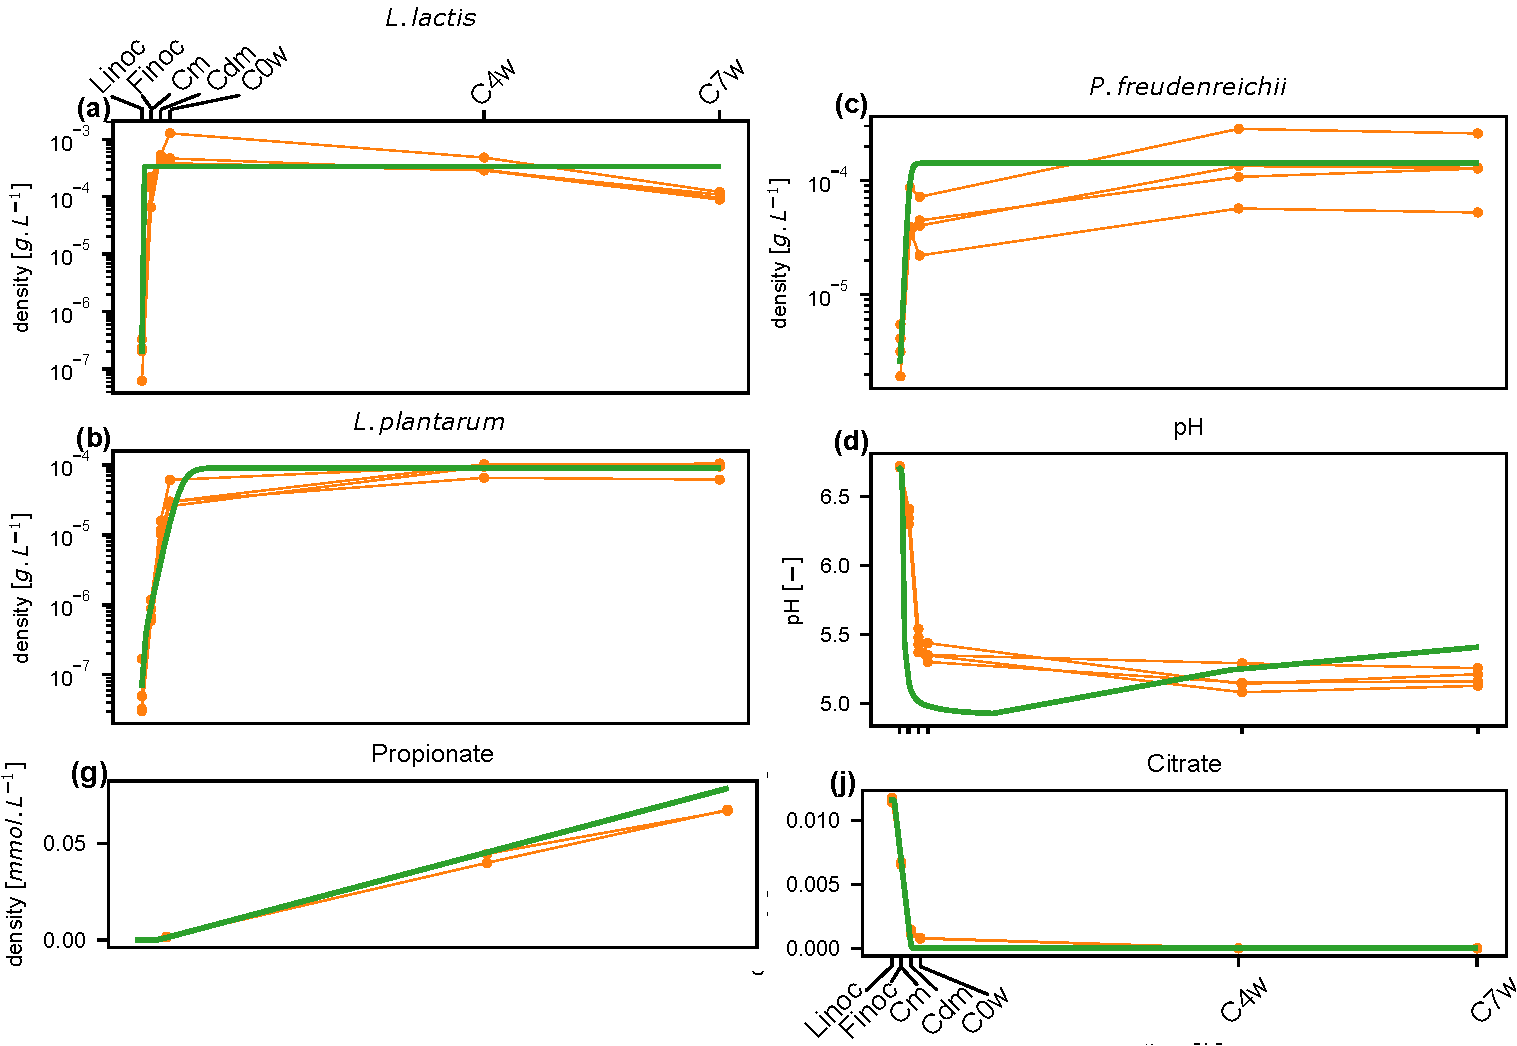
\includegraphics[width=0.8\textwidth]{figures/community-pred-growth.pdf}
\begin{block}{}
\begin{itemize}
\item Growth well predicted for all bacteria
\item Lactate proxy production can explain the observed pH
\item Metabolomic data is well predicted 
\end{itemize}
\end{block}
\end{frame}


\begin{frame}
\frametitle{Highlighted bacterial community behavior}
\centering
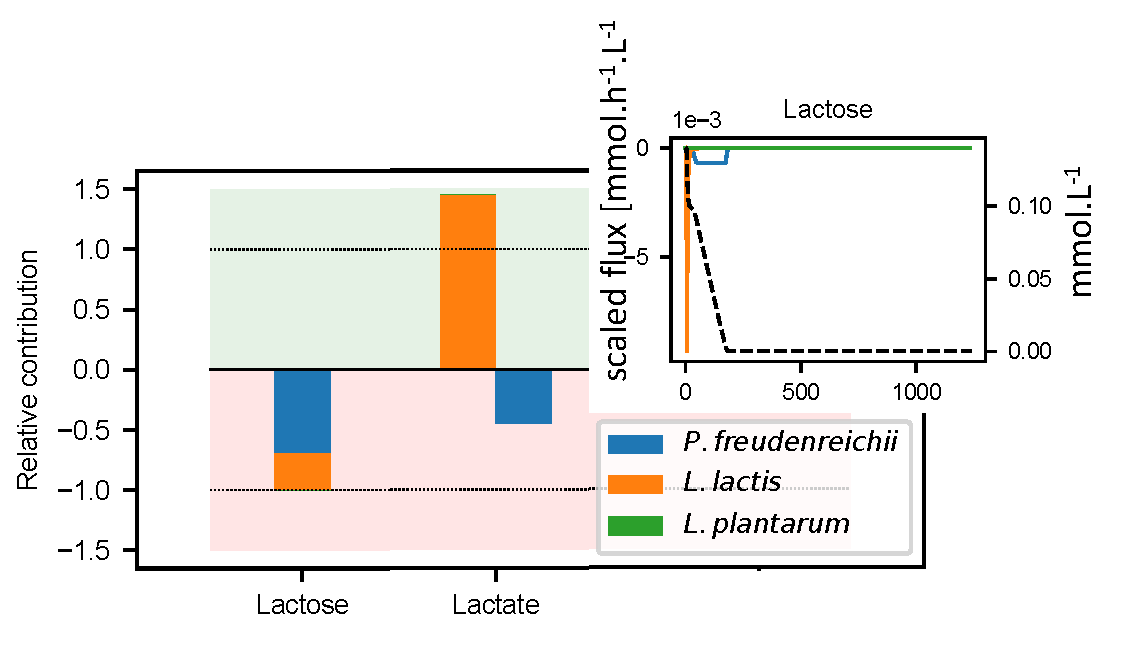
\includegraphics[width=0.8\textwidth]{figures/relative-contribution.pdf}
\begin{minipage}{0.5\textwidth}

\begin{itemize}
\item Temporal segregation for lactose
\item \textit{L. lactis} main lactate producer 
\item Commensalism between \lactis and \freud
\end{itemize}

\end{minipage}%
\begin{minipage}{0.5\textwidth}
\begin{itemize}
\item 11 shared metabolites predicted with SMETANA, MiCOM (phenylalanine, succinate, xanthine..)
\end{itemize}
\end{minipage}

\footcite{Zelezniak2015,diener2020}
\end{frame}


\begin{frame}
\frametitle{Numerical model conclusion}
\centering
\textbf{\huge Numerical modelling of a controlled community}

\begin{minipage}{0.45\textwidth}
\vspace{0.3cm}
\begin{block}{Strength}
\begin{itemize}
\item Faithful numerical model on small communities %
\item Iterative process (refinement and calibration)
\end{itemize}
\end{block} %
\end{minipage}\hfill
\hspace{0.5cm}
\hfill
\begin{minipage}{0.45\textwidth}
\begin{block}{Weaknesses}
\begin{itemize}
\item Greedy process
\item \textit{A priori} knowledge
\end{itemize}
\end{block}

\end{minipage}


\begin{minipage}{0.45\textwidth}
\begin{block}{Opportunities}
In silico model usable in industrial contexts
\end{block} %
\end{minipage}\hfill
\hspace{0.5cm}
\hfill
\begin{minipage}{0.45\textwidth}
\begin{block}{Threats}
Scalability
\end{block}
\end{minipage}

%
%\begin{minipage}{0.45\textwidth}
%\begin{block}{Originality}
%\begin{itemize}
%\item High quality of refinement and well calibrated individual GSMN from cheese %
%\item Individual calibrations based on community behavior permit the prediction metabolites concentrations %
%\end{itemize}
%\end{block} %
%\end{minipage}\hfill
%\hspace{0.5cm}
%\hfill
%\begin{minipage}{0.45\textwidth}
%\begin{block}{Scalability issue}
%\begin{itemize}
%\item Refinement process is time consuming
%\item The iterative methodology assume well documented GSMNs in literature
%\item Based on \textit{a priori} knowledge for screening compounds
%\end{itemize}
%\end{block}
%\end{minipage}

%\begin{block}{Solution}
%For screening large community, use of different formalism is required
%\end{block}


\end{frame}

\section{Discrete model}

%\begin{frame}
%\frametitle{Characterization of large-scale bacterial communities}
%\begin{figure}
%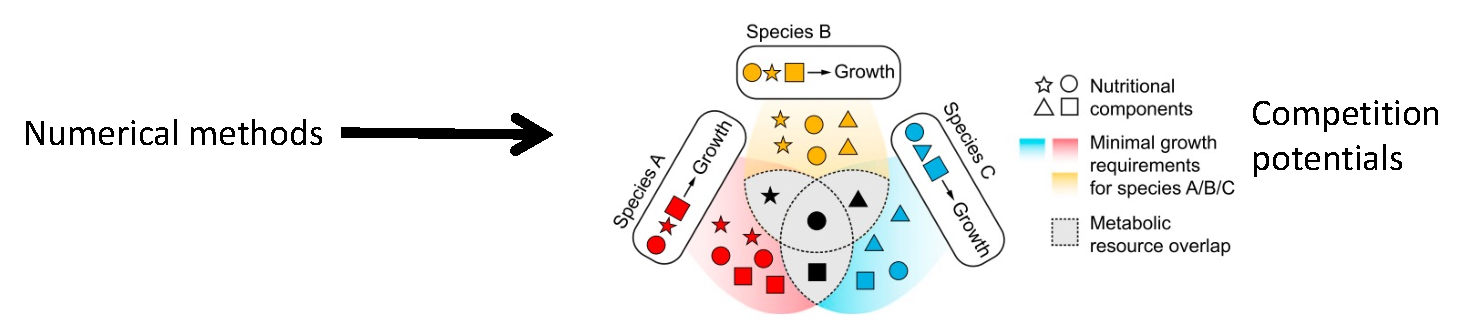
\includegraphics[width=\textwidth]{figures/sota-num.pdf}
%\end{figure}
%\begin{block}{}
%\begin{itemize}
%\item Community size analysis up to 18 \normalsize in a reasonable time (SMETANA)
%\end{itemize}
%\end{block}
%\begin{figure}
%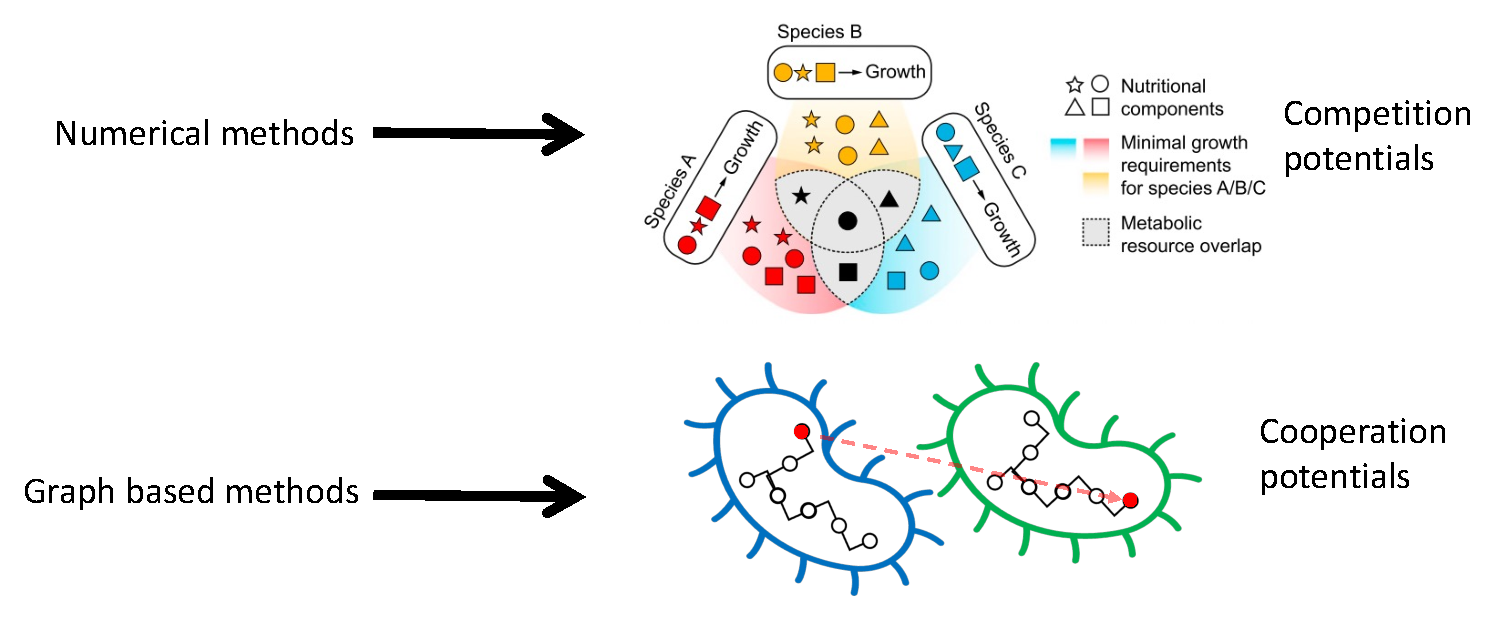
\includegraphics[width=\textwidth]{figures/sota-discrete.pdf}
%\end{figure}
%\begin{block}{}
%\begin{itemize}
%\item Tedious pairwise analysis for graph base methods (NetCoop)
%\item Discrete-based methods not limited by the size of community 
%\end{itemize}
%\end{block}
%\footcite{Zelezniak2015,Levy2015}
%\end{frame}

\begin{frame}
\frametitle{Discrete approach for characterizing large-scale bacterial interaction}
\centering
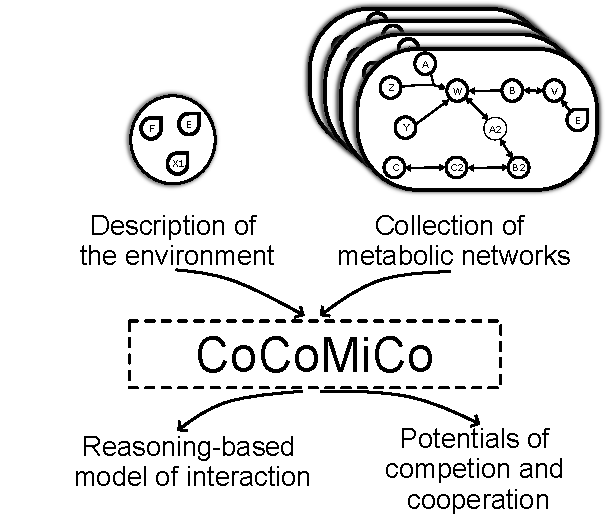
\includegraphics[width=0.55\textwidth]{figures/concept.pdf}

\begin{minipage}{0.5\textwidth}
\vspace{-0.3cm}
\begin{block}{Challenge}
\begin{itemize}
\item Scalable to natural environment 
\item Whole community
\item Define cooperation and competition
\item Characterize metabolic interaction properties 
\end{itemize}
\end{block}
\end{minipage}%
\hspace{0.2cm}
\hfill
\begin{minipage}{0.45\textwidth}
\vspace{-0.3cm}
\begin{alertblock}{Solution}
\begin{itemize}
\item Create a discrete approach (reasoning-based)
\item Create a consistent KB and rules
\item CoCoMiCo implementation for characterizing bacterial interactions
\end{itemize}
\end{alertblock}
\end{minipage}

\end{frame}

\begin{frame}
\frametitle{KB and logical rules constructions}
\begin{itemize}
\item Report relations between metabolites and reactions
\end{itemize}
\textbf{Source of the KB}
\begin{minipage}{0.5\textwidth}
\hspace{-0.15\textwidth}
\begin{tikzpicture}
   \node (x) [circle, draw] at (0,0)   {X};
   \node (a) [circle, draw] at (2,0)   {A};
   \node (b) [circle, draw] at (4,0)   {C};
   \node (c) [circle, draw] at (3,1)   {D};
   \node (d) [circle, draw] at (5,-1)   {E};
   \node (e) [circle, draw] at (3.5,-2)   {F};
          
    \node (f) [rectangle, draw] at (1,0) {$r_1$};
  	\node (g) [rectangle, draw] at (3,0)  {$r_2$};
  	\node (h) [rectangle, draw] at (5,0)   {$r_3$};
  	\node (i) [rectangle, draw] at (4,-1)   {$r_4$};
  	\node (j) [rectangle, draw] at (5,-2)   {$r_5$};

    \graph { (x) -> (f) -> (a) };
    \graph { (x) -> (f) -> (c) };
    \graph { (a) -> (g) -> (c) };
    \graph { (a) -> (g) -> (b) };
	\graph { (b) -> (h) <-> (c) };
	\graph { (b) -> (h) -> (d) };            
	\graph { (b) <- (i) <- (d) };       
	\graph { (d) <- (j) <- (e) };               
	
	     \draw [draw=black] (0.5,1.5) rectangle (5.5,-2.5);     
     
     \node (extracellular) [] at (5.1,1.75) {\tiny \textit{extracellular}};
     \node (intracellular) [] at (4.5,1.25) {\tiny \textit{intracellular}};	

\end{tikzpicture}
\end{minipage}%
\begin{minipage}{0.55\textwidth}
\vspace{-1.6cm}\textbf{Source of the rules}
\begin{block}{}
Modeler and biological expert
\end{block}
\begin{itemize}
\item Producibility is initiated by the presence of nutrients,
\item The products of a reactions are producible if all reactants of this reaction are themselves producible
\end{itemize}
\end{minipage}
\begin{alertblock}{}
The scope, \textit{i.e.} the metabolic capacity of a network reasons on the biochemical reactions
\end{alertblock}
\footcite{Ebenhoh2004}
\end{frame}

\begin{frame}
\frametitle{Illustration of the scope}

\only<1>{
\begin{minipage}{0.5\textwidth}
\hspace{-0.15\textwidth}
\begin{tikzpicture}
   \node (x) [circle, draw,fill=black!30!yellow] at (0,0)   {X};
   \node (a) [circle, draw,fill=white!60!yellow] at (2,0)   {A};
   \node (b) [circle, draw] at (4,0)   {C};
   \node (c) [circle, draw,fill=white!60!yellow] at (3,1)   {D};
   \node (d) [circle, draw] at (5,-1)   {E};
   \node (e) [circle, draw] at (3.5,-2)   {F};
          
    \node (f) [rectangle, draw,fill=white!60!yellow] at (1,0) {$r_1$};
  	\node (g) [rectangle, draw] at (3,0)  {$r_2$};
  	\node (h) [rectangle, draw] at (5,0)   {$r_3$};
  	\node (i) [rectangle, draw] at (4,-1)   {$r_4$};
  	\node (j) [rectangle, draw] at (5,-2)   {$r_5$};

    \graph { (x) -> (f) -> (a) };
    \graph { (x) -> (f) -> (c) };
    \graph { (a) -> (g) -> (c) };
    \graph { (a) -> (g) -> (b) };
	\graph { (b) -> (h) <-> (c) };
	\graph { (b) -> (h) -> (d) };            
	\graph { (b) <- (i) <- (d) };             
	\graph { (d) <- (j) <- (e) };    
	    \graph { (e) -> (i) };
	
	     \draw [draw=black] (0.5,1.5) rectangle (5.5,-2.5);     
	     
     \node (extracellular) [] at (5.1,1.75) {\tiny \textit{extracellular}};
     \node (intracellular) [] at (4.5,01) {\tiny \textit{intracellular}};	
 \end{tikzpicture}
\end{minipage}%
\begin{minipage}{0.55\textwidth}
\begin{block}{}
Modeler and biological expert
\end{block}
\begin{itemize}
\item Producibility is initiated by the presence of nutrients,
\item The products of a reactions are producible if all reactants of this reaction are themselves producible
\end{itemize}
X is a seed \\
scope : X,A,D
\end{minipage}


}


\only<2>{
\begin{minipage}{0.5\textwidth}
\hspace{-0.15\textwidth}
\begin{tikzpicture}
   \node (x) [circle, draw,fill=black!30!yellow] at (0,0)   {X};
   \node (a) [circle, draw,fill=white!60!yellow] at (2,0)   {A};
   \node (b) [circle, draw,fill=white!60!yellow] at (4,0)   {C};
   \node (c) [circle, draw,fill=white!60!yellow] at (3,1)   {D};
   \node (d) [circle, draw] at (5,-1)   {E};
   \node (e) [circle, draw] at (3.5,-2)   {F};
          
    \node (f) [rectangle, draw,fill=white!60!yellow] at (1,0) {$r_1$};
  	\node (g) [rectangle, draw,fill=white!60!yellow] at (3,0)  {$r_2$};
  	\node (h) [rectangle, draw] at (5,0)   {$r_3$};
  	\node (i) [rectangle, draw] at (4,-1)   {$r_4$};
  	\node (j) [rectangle, draw] at (5,-2)   {$r_5$};

    \graph { (x) -> (f) -> (a) };
    \graph { (x) -> (f) -> (c) };
    \graph { (a) -> (g) -> (c) };
    \graph { (a) -> (g) -> (b) };
	\graph { (b) -> (h) <-> (c) };
	\graph { (b) -> (h) -> (d) };            
	\graph { (b) <- (i) <- (d) };         
	\graph { (d) <- (j) <- (e) };               
	    \graph { (e) -> (i) };
	
	     \draw [draw=black] (0.5,1.5) rectangle (5.5,-2.5);     
	     
     \node (extracellular) [] at (5.1,1.75) {\tiny \textit{extracellular}};
     \node (intracellular) [] at (4.5,01) {\tiny \textit{intracellular}};	
\end{tikzpicture}
\end{minipage}%
\begin{minipage}{0.55\textwidth}

\begin{block}{}
Modeler and biological expert
\end{block}
\begin{itemize}
\item Producibility is initiated by the presence of nutrients,
\item The products of a reactions are producible if all reactants of this reaction are themselves producible
\end{itemize}
X is a seed \\
scope : X,A,D,C
\end{minipage}


}



\only<3>{

\begin{minipage}{0.5\textwidth}
\hspace{-0.15\textwidth}
\begin{tikzpicture}
   \node (x) [circle, draw,fill=black!30!yellow] at (0,0)   {X};
   \node (a) [circle, draw,fill=white!60!yellow] at (2,0)   {A};
   \node (b) [circle, draw,fill=white!60!yellow] at (4,0)   {C};
   \node (c) [circle, draw,fill=white!60!yellow] at (3,1)   {D};
   \node (d) [circle, draw,fill=white!60!yellow] at (5,-1)   {E};
   \node (e) [circle, draw] at (3.5,-2)   {F};
          
    \node (f) [rectangle, draw,fill=white!60!yellow] at (1,0) {$r_1$};
  	\node (g) [rectangle, draw,fill=white!60!yellow] at (3,0)  {$r_2$};
  	\node (h) [rectangle, draw,fill=white!60!yellow] at (5,0)   {$r_3$};
  	\node (i) [rectangle, draw] at (4,-1)   {$r_4$};
  	\node (j) [rectangle, draw] at (5,-2)   {$r_5$};
  	


    \graph { (x) -> (f) -> (a) };
    \graph { (x) -> (f) -> (c) };
    \graph { (a) -> (g) -> (c) };
    \graph { (a) -> (g) -> (b) };
	\graph { (b) -> (h) <-> (c) };
	\graph { (b) -> (h) -> (d) };            
	\graph { (b) <- (i) <- (d) };           
	\graph { (d) <- (j) <- (e) };    
    \graph { (e) -> (i) };    
	
	     \draw [draw=black] (0.5,1.5) rectangle (5.5,-2.5);     
	     
     \node (extracellular) [] at (5.1,1.75) {\tiny \textit{extracellular}};
     \node (intracellular) [] at (4.5,01) {\tiny \textit{intracellular}};	
\end{tikzpicture}
\end{minipage}%
\begin{minipage}{0.55\textwidth}

\begin{block}{}
Modeler and biological expert
\end{block}
\begin{itemize}
\item Producibility is initiated by the presence of nutrients,
\item The products of a reactions are producible if all reactants of this reaction are themselves producible
\end{itemize}
X is a seed \\
scope : X,A,D,C,E
\end{minipage}

}
\end{frame}

\begin{frame}[fragile]
\frametitle{KB and logical rules constructions}
\begin{onlyenv}<1>
\begin{itemize}
\item Report relations between metabolites and reactions
\end{itemize}
\textbf{Source of the KB}
\begin{minipage}{0.5\textwidth}
\hspace{-0.15\textwidth}
\begin{tikzpicture}
   \node (x) [circle, draw] at (0,0)   {X};
   \node (a) [circle, draw] at (2,0)   {A};
   \node (b) [circle, draw] at (4,0)   {C};
   \node (c) [circle, draw] at (3,1)   {D};
   \node (d) [circle, draw] at (5,-1)   {E};
   \node (e) [circle, draw] at (3.5,-2)   {F};

    \node (f) [rectangle, draw] at (1,0) {$r_1$};
  	\node (g) [rectangle, draw] at (3,0)  {$r_2$};
  	\node (h) [rectangle, draw] at (5,0)   {$r_3$};
  	\node (i) [rectangle, draw] at (4,-1)   {$r_4$};
  	\node (j) [rectangle, draw] at (5,-2)   {$r_5$};

    \graph { (x) -> (f) -> (a) };
    \graph { (x) -> (f) -> (c) };
    \graph { (a) -> (g) -> (c) };
    \graph { (a) -> (g) -> (b) };
	\graph { (b) -> (h) <-> (c) };
	\graph { (b) -> (h) -> (d) };
	\graph { (b) <- (i) <- (d) };
	\graph { (d) <- (j) <- (e) };
	
	     \draw [draw=black] (0.5,1.5) rectangle (5.5,-2.5);

     \node (extracellular) [] at (5.1,1.75) {\tiny \textit{extracellular}};
     \node (intracellular) [] at (4.5,1.25) {\tiny \textit{intracellular}};	

\end{tikzpicture}
\end{minipage}%
\begin{minipage}{0.55\textwidth}
\vspace{-.1cm}
\textbf{Source of the rules}
\begin{block}{}
Modeler and biological expert
\end{block}
\begin{itemize}
\item Producibility is initiated by the presence of nutrients,
\item The products of a reactions are producible if all reactants of this reaction are themselves producible
\end{itemize}

\begin{lstlisting}[style=asp]
scope(M) :- seed(M).
scope(M) :- bacteria(B), product(M,R,B), reaction(R,B), scope(M2) : reactant(M2,R,B).
\end{lstlisting}
\end{minipage}

\begin{alertblock}{}
The scope of a network is formalized in 2 logical rules
\end{alertblock}

\end{onlyenv}

\begin{onlyenv}<2>
\begin{itemize}
\item Report relations between metabolites and reactions
\end{itemize}
\textbf{Source of the KB}
\begin{minipage}{0.5\textwidth}
\hspace{-0.15\textwidth}
\begin{tikzpicture}
   \node (x) [circle, draw] at (0,0)   {X};
   \node (a) [circle, draw] at (2,0)   {A};
   \node (b) [circle, draw] at (4,0)   {C};
   \node (c) [circle, draw] at (3,1)   {D};
   \node (d) [circle, draw] at (5,-1)   {E};
   \node (e) [circle, draw] at (3.5,-2)   {F};

    \node (f) [rectangle, draw] at (1,0) {$r_1$};
  	\node (g) [rectangle, draw] at (3,0)  {$r_2$};
  	\node (h) [rectangle, draw] at (5,0)   {$r_3$};
  	\node (i) [rectangle, draw] at (4,-1)   {$r_4$};
  	\node (j) [rectangle, draw] at (5,-2)   {$r_5$};

    \graph { (x) -> (f) -> (a) };
    \graph { (x) -> (f) -> (c) };
    \graph { (a) -> (g) -> (c) };
    \graph { (a) -> (g) -> (b) };
	\graph { (b) -> (h) <-> (c) };
	\graph { (b) -> (h) -> (d) };
	\graph { (b) <- (i) <- (d) };
	\graph { (d) <- (j) <- (e) };
	
	     \draw [draw=black] (0.5,1.5) rectangle (5.5,-2.5);

     \node (extracellular) [] at (5.1,1.75) {\tiny \textit{extracellular}};
     \node (intracellular) [] at (4.5,1.25) {\tiny \textit{intracellular}};	

\end{tikzpicture}
\end{minipage}%
\begin{minipage}{0.55\textwidth}
\vspace{-.1cm}
\textbf{Source of the rules}
\begin{block}{}
Modeler and biological expert
\end{block}
\begin{itemize}
\item Producibility is initiated by the presence of nutrients,
\item The products of a reactions are producible if all reactants of this reaction are themselves producible
\end{itemize}

\begin{lstlisting}[style=asp]
scope(metabolite(M,B), Community) :-
		taxon(B),
		in_community(Community, B),
		reaction(R,B),
		product(M,R,B),
		available(M', Community) : reactant(M',R,B).

available(M, Community) :- seed(M), community(Community).
available(M, Community) :- scope(metabolite(M,B), Community).

\end{lstlisting}
\end{minipage}
\end{onlyenv}

%\begin{alertblock}{}
%Answer Set Programming as a logical formalism encoding the scope
%\end{alertblock}
\footcite{Ebenhoh2004}

\end{frame}

\begin{frame}
\frametitle{Answer Set Programming formalism}
\centering
\begin{figure}[h]
\includegraphics[width=\textwidth]{figures/asp.pdf}
\caption{The workflow of Answer set programming (ASP)}
\end{figure}
\begin{block}{}
\begin{itemize}
\item Closed world assumption $\rightarrow$ unknown information is false
\item Mechanistic model
\item Solve combinatorial problems
\end{itemize}

\end{block}
\footcite{Kaufmann2016GroundingAS}
\end{frame}

\begin{frame}
\frametitle{Challenge: Characterize cooperation properties}
\only<1>{
%\hspace{-0.5cm}
\begin{minipage}{0.4\textwidth}
\begin{block}{Cooperation properties}
\begin{itemize}
\item Exchanged metabolites
\end{itemize}
\end{block}
\end{minipage}%
\hspace{0.5cm}
\hfill
\begin{minipage}{0.45\textwidth}
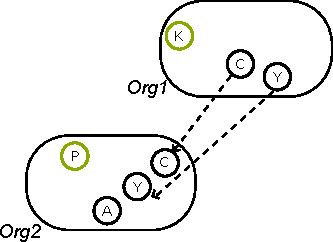
\includegraphics[width=\textwidth]{figures/properties-2.pdf}
\end{minipage}

\begin{alertblock}{}
\begin{itemize}
\item Redesigned microbial ecology definition of cooperation $\rightarrow$  no growth effect
\item Effect on donors are not taken into account (0, +, -)
\end{itemize}
\end{alertblock}
}

\only<2>{
%\hspace{-0.5cm}
\begin{minipage}{0.4\textwidth}
\begin{block}{Cooperation properties}
\begin{itemize}
\item Exchanged metabolites
\item Can a species give to everyone in the system ?
\end{itemize}
\end{block}
\end{minipage}%
\hspace{0.5cm}
\hfill
\begin{minipage}{0.45\textwidth}
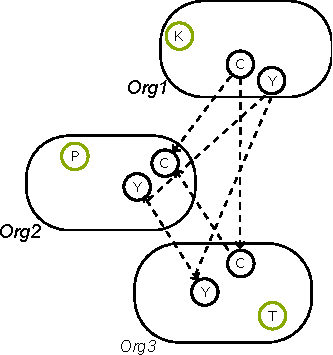
\includegraphics[width=\textwidth]{figures/properties.pdf}
\end{minipage}
}

\only<3>{

\begin{minipage}{0.4\textwidth}
\begin{block}{Cooperation properties}
\begin{itemize}
\item Exchanged metabolites
\item Can a species give to everyone in the system ?
\item Added-value of adding a species
\end{itemize}
\end{block}
\end{minipage}%
\hspace{0.5cm}
\hfill
\begin{minipage}{0.45\textwidth}
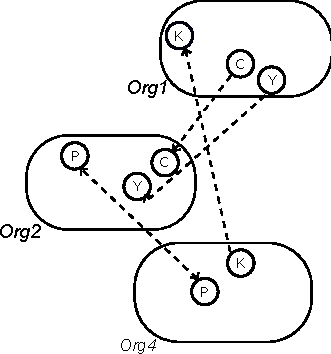
\includegraphics[width=\textwidth]{figures/properties-4.pdf}
\end{minipage}


}

\only<4>{
\begin{minipage}{0.4\textwidth}
\begin{block}{Cooperation properties}
\begin{itemize}
\item Exchanged metabolites
\item Can a species give to everyone in the systeme ?
\item Added-value of adding a species
\item Compare cooperation indexes 
\end{itemize}
\end{block}
\end{minipage}%
\hspace{0.5cm}
\hfill
\begin{minipage}{0.45\textwidth}
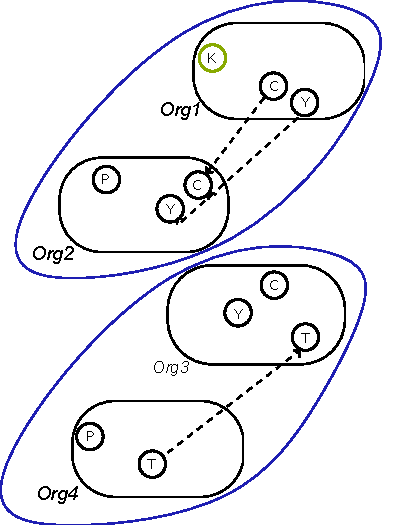
\includegraphics[width=\textwidth]{figures/properties-3.pdf}
\end{minipage}
}

\end{frame}

\begin{frame}
\frametitle{Characterize competition interaction, economic point of view}
\only<1>{
\begin{minipage}{0.4\textwidth}
\begin{itemize}
\item Monopsony
\end{itemize}
 Monopsony comes from two Greek words: ``monos'' meaning ``single'' and ``opsonia'' meaning ``purchase.''
\end{minipage}%
\hspace{0.5cm}
\hfill
\begin{minipage}{0.45\textwidth}
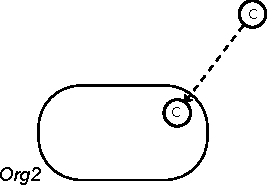
\includegraphics[width=0.7\textwidth]{figures/monopsonie.pdf}
\end{minipage}
}

\only<2>{
\begin{minipage}{0.4\textwidth}
\begin{itemize}
\item Monopsony
\end{itemize}
 Monopsony comes from two Greek words: ``monos'' meaning ``single'' and ``opsonia'' meaning ``purchase.''
\end{minipage}%
\hspace{0.5cm}
\hfill
\begin{minipage}{0.45\textwidth}
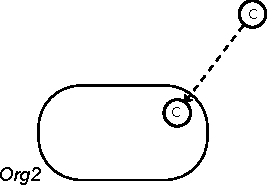
\includegraphics[width=0.7\textwidth]{figures/monopsonie.pdf}
\end{minipage}
\begin{minipage}{0.4\textwidth}
\begin{itemize}
\item \textbf{Polyopsony}
\end{itemize}
\end{minipage}%
\hspace{0.5cm}
\hfill
\begin{minipage}{0.45\textwidth}
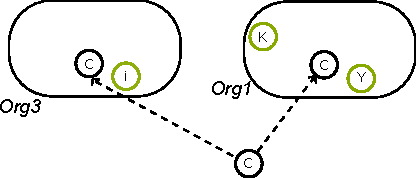
\includegraphics[width=\textwidth]{figures/polyopsonie.pdf}
\end{minipage}


\begin{block}{}
\begin{itemize}
\item How cooperation and competition (polyopsony) rules are defined ?
\end{itemize}
\end{block}
}




\end{frame}



%
%\begin{frame}
%\frametitle{Cooperation \& competition properties}
%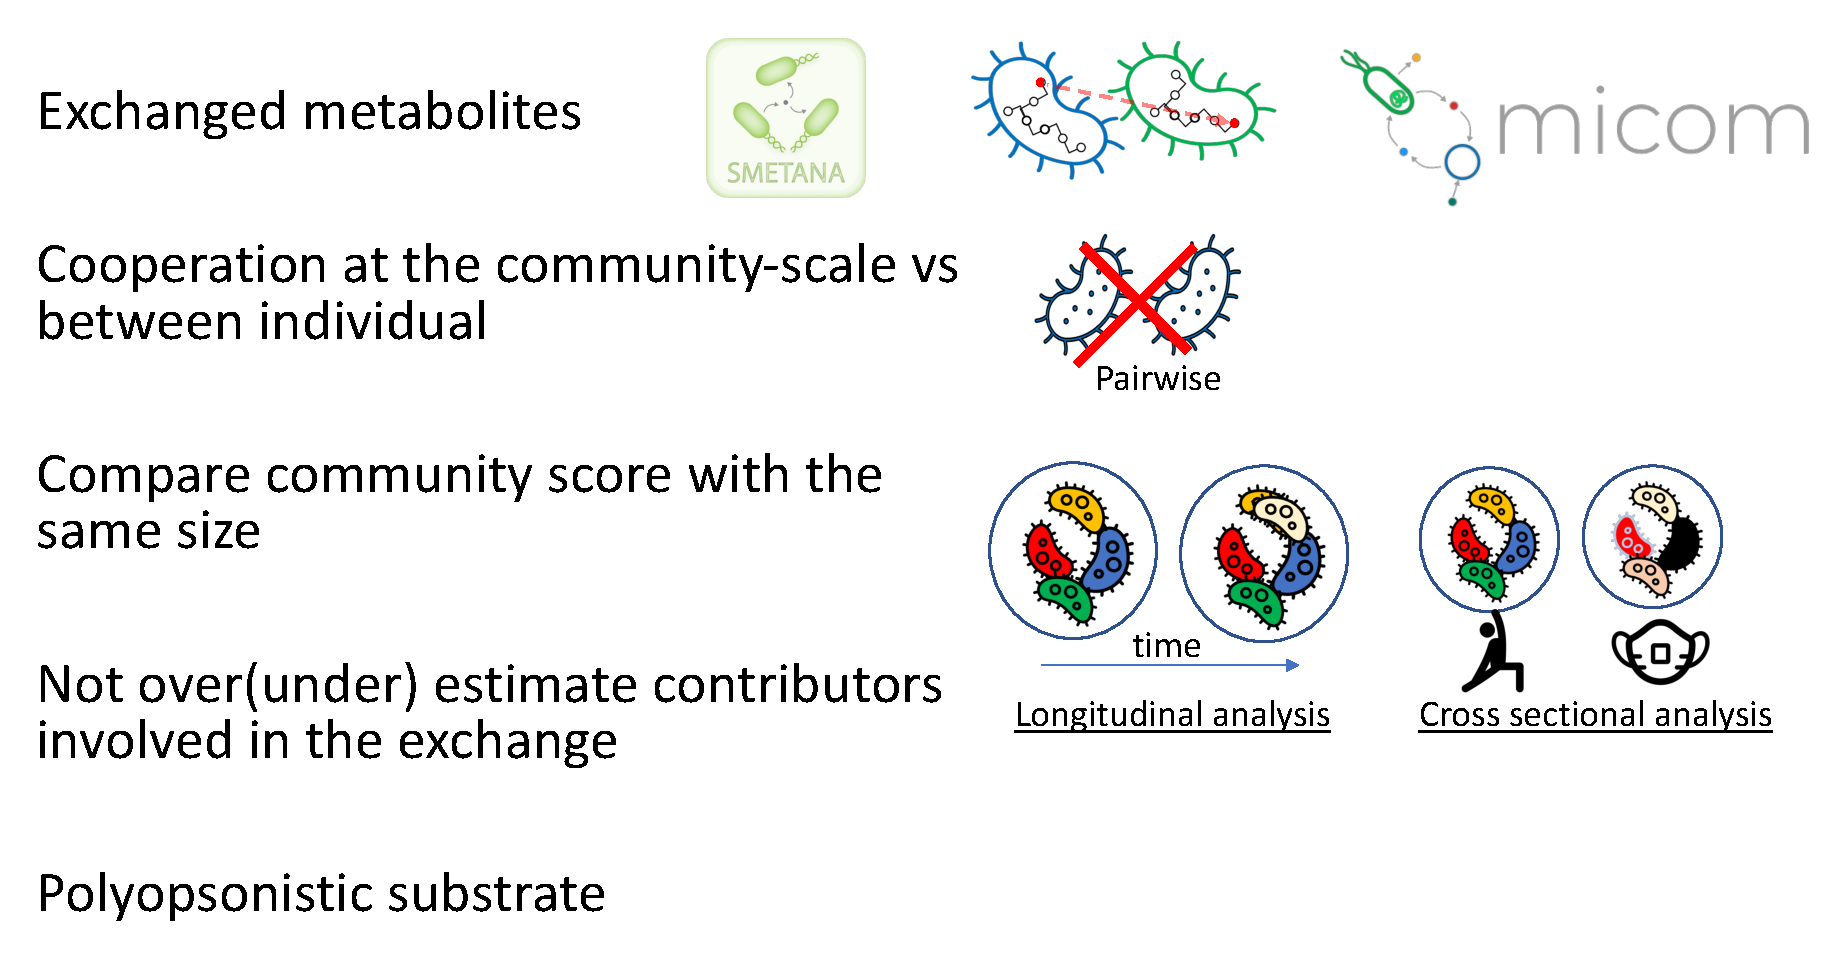
\includegraphics[width=\textwidth]{figures/coop-properties.pdf}
%\begin{block}{}
%\begin{itemize}
%\item Inference of polyopsonistic substrate and exchanged compounds in logical rules (ASP)
%\item Index of cooperation and competition in python
%\end{itemize}
%\end{block}
%\end{frame}


\begin{frame}[fragile]
\frametitle{Potential interactions rules}
\begin{onlyenv}<1>
\begin{minipage}{0.5\textwidth}
\begin{lstlisting}[mathescape=True, label={lst:echange}] captionpos=b,style=aspwide]
exchange(M,P,C) :- taxon(P),
taxon(C),
P != C,
reactant(M,_,C),
product(M,_,P),
scope(metabolite(M,P),
 all),
not scope(metabolite(M,C), 
self(C)).
\end{lstlisting}
%\begin{itemize}
%	\item[ligne 1:] un métabolite \texttt{M} est échangeable entre un producteur \texttt{P} et un consommateur \texttt{C} si \texttt{P} est un taxon et 
%	\item[ligne 2:] que \texttt{C} est un taxon et
%	\item[ligne 3:] \texttt{P} est différent de \texttt{C} et
%	\item[ligne 4:] que \texttt{M} est un réactant de n'importe quelle réaction de \texttt{C} et 
%	\item[ligne 5:] que \texttt{M} est un produit de n'importe quelle réaction de \texttt{P} et
%	\item[ligne 6:] que \texttt{M} est dans le \texttt{scope} communautaire produit par \texttt{P} et 
%	\item[ligne 7:] que \texttt{M} n'est pas dans le \texttt{scope} de \texttt{C}.
%\end{itemize}
\end{minipage}%
\hspace{0.25cm}
\hfill
\begin{minipage}{0.45\textwidth}
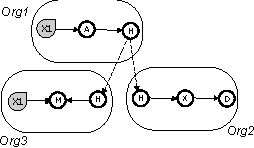
\includegraphics[width=\textwidth]{figures/exchanged.pdf}
\end{minipage}
\end{onlyenv}

\begin{onlyenv}<2>
\begin{minipage}{0.5\textwidth}
\begin{lstlisting}[mathescape=True, label={lst:echange}] captionpos=b,style=aspwide]
exchange(M,P,C) :- taxon(P),
taxon(C),
P != C,
reactant(M,_,C),
product(M,_,P),
scope(metabolite(M,P),
 all),
not scope(metabolite(M,C), 
self(C)).
\end{lstlisting}
\begin{lstlisting}[mathescape=True,label={lst:competition}, captionpos=b]
polyopsony(M,N) :- 
N=#count{C,M:exchange(M,_,C)},
exchange(M,_,_), N > 1.
		 	
polyopsony(S,N) :-
N=#count{B:seed_consumed_by_taxon(S,B)}, 
N > 1, seed(S).
\end{lstlisting}
%\begin{itemize}
%	\item[ligne 2-3:] Un composé échangé \texttt{M} est limitant si lorsque le nombre de consommateurs \texttt{C} impliqués dans l'échange de ce métabolite \texttt{M} est strictement supérieur à 1.
%	\item[ligne 6-7:] Une graine \texttt{M} est considérée limitante lorsque le nombre de consommateurs \texttt{C} de cette graine \texttt{M} est strictement supérieur à 1. \\
%\end{itemize}
\end{minipage}%
\hspace{0.25cm}
\hfill
\begin{minipage}{0.45\textwidth}
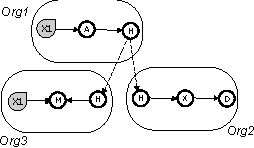
\includegraphics[width=\textwidth]{figures/exchanged.pdf}
\end{minipage}
\end{onlyenv}
\end{frame}

\begin{frame}
\frametitle{Scope of CoCoMiCo}

\textbf{Use of logical formalism for characterizing cooperation and competition properties}
\begin{itemize}
\item \textit{Exchanged compounds}
\item Polyopsony, monopsony
\item Bacteria involved in an exchange
\item $\rho, \delta $ metrics  
\end{itemize}

\vspace{1cm}
\textbf{ Calculate indexes of cooperation and competition}
\begin{itemize}
\item Compare communities
\item Use as optimization criteria 
\end{itemize}

\begin{alertblock}{}
Cooperation (exchanged compounds) and competition (polyopsony) properties used for calculating cooperation and competition indexes
\end{alertblock}

\footcite{Frioux2018}
\end{frame}

\begin{frame}[fragile]
\frametitle{Cooperation  indexes}


\begin{minipage}{0.5\textwidth}
\begin{block}{Cooperation weight}
Can a species give to everyone in the systeme ? \\
How to qualitatively model the contributions of exchange species?
\end{block}
\textbf{Exchangeable metabolites}\\
\begin{lstlisting}[mathescape=True]
H:{Org1} % producer
H:{Org2,Org3} % consumers
\end{lstlisting}


\[
w(k) = 2-{0.5^{k-1}}
\]


\begin{lstlisting}[mathescape=True]
H:{1} % producer
H:{1.5} % consumers
\end{lstlisting}
\[
\begin{split}
    \textsf{CooP} &= \sum_{m\in M} w(|P_m|) + \sum_{m\in M} w(|C_m|)\\
      &=  2.5
\end{split}
\]


\end{minipage}%
\hspace{0.5cm}
\hfill
\begin{minipage}{0.4\textwidth}
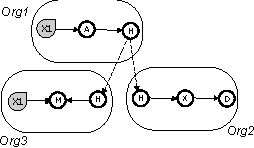
\includegraphics[width=\textwidth]{figures/exchanged.pdf}
\end{minipage}
\end{frame}


\begin{frame}[fragile]
%\begin{onlyenv}<2>
\frametitle{Competition  indexes}
\begin{minipage}{0.5\textwidth}

\begin{exampleblock}{Polyopsonistic}
Number of consumers involved in exchangeable metabolites and seed > 1
\end{exampleblock}{}

\begin{lstlisting}[mathescape=True]
H:{Org2,Org3} % exchanged metabolite
X1:{Org1} %  the nutrient
\end{lstlisting}

\begin{lstlisting}[mathescape=True]
 Comp = sum(polyopsonist.values())) / len(community.taxa)
      = 2/3
\end{lstlisting}

%\begin{exampleblock}{$\rho$}
%Identify the reactionary added-value between the reaction scope in community and individually
%\end{exampleblock}{}
%
%\begin{exampleblock}{$\delta$}
%Identify the producible compounds added-value between the metabolite scope in community and individually
%\end{exampleblock}{}

\end{minipage}%
\hspace{0.5cm}
\hfill
\begin{minipage}{0.4\textwidth}
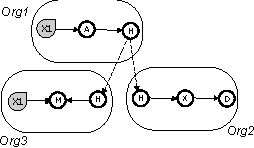
\includegraphics[width=\textwidth]{figures/exchanged.pdf}
\end{minipage}
%\end{onlyenv}


\end{frame}




\begin{frame}
\frametitle{Workflow for method assessment}

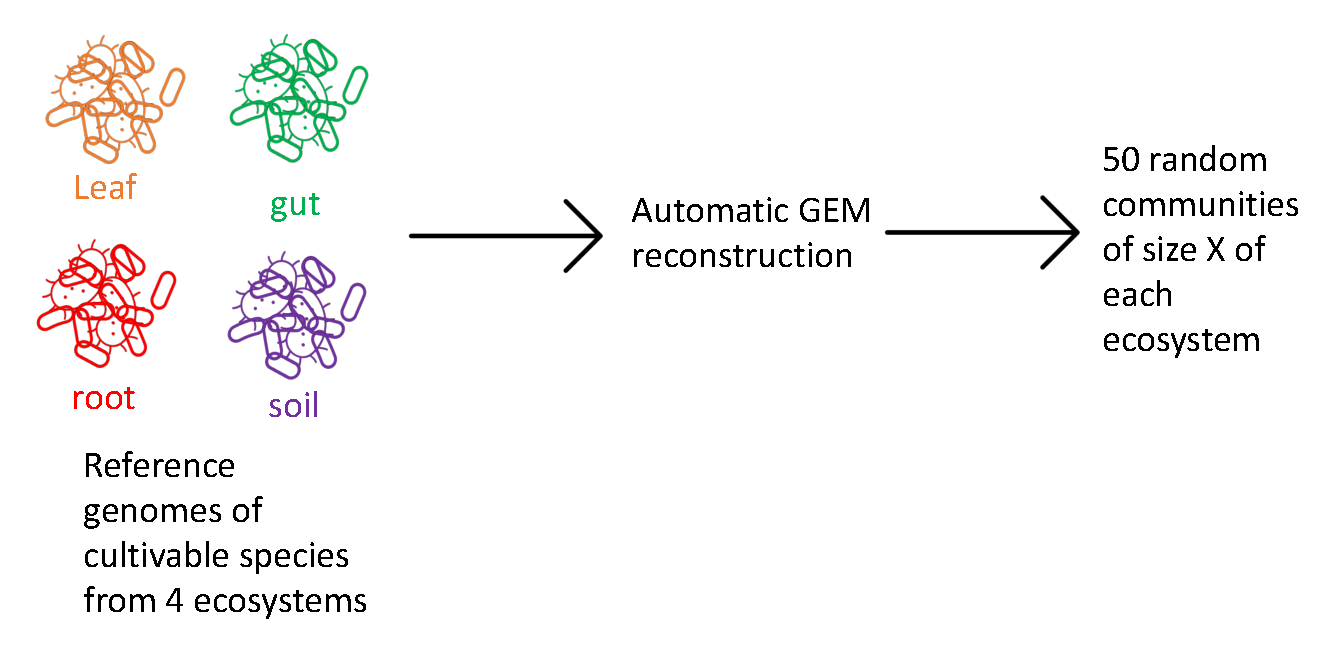
\includegraphics[width=\textwidth]{figures/workflow-ccmc.pdf}

\begin{block}{Goal}
\begin{itemize}
\item Ecosystem consistency
\item Added-value of removing/adding species
\end{itemize}
\end{block}

\end{frame}


\begin{frame}
\frametitle{Are scores ecosystem consistent?}
%\begin{minipage}{0.65\textwidth}
%\textbf{Generic seeds}
%\begin{figure}
%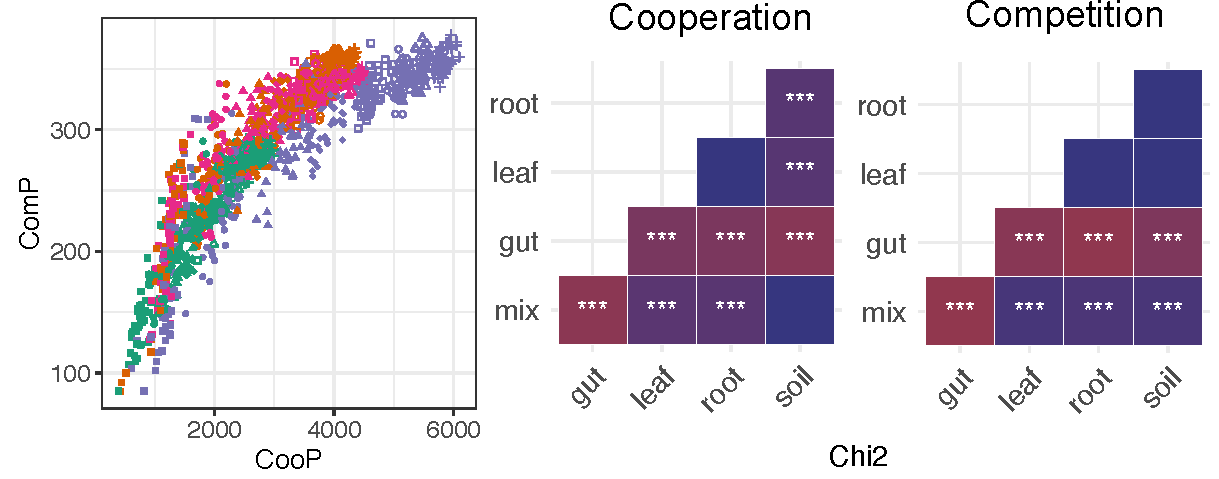
\includegraphics[width=\textwidth]{figures/coop-comp-ecosys.pdf}
%\end{figure}
\textbf{Specific seeds}
\begin{figure}
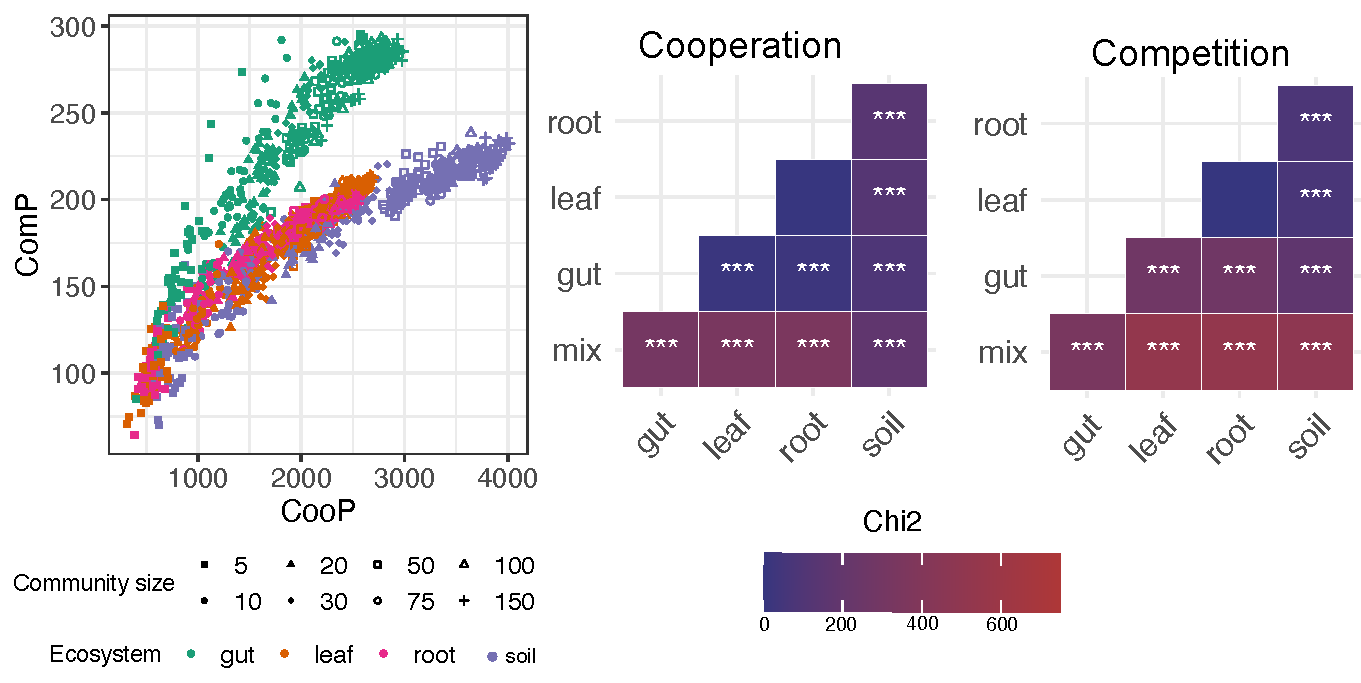
\includegraphics[width=\textwidth]{figures/coop-comp-ecosys-specific.pdf}
\end{figure}
%\end{minipage}
%\hspace{0.1cm}
%\hfill
%\begin{minipage}{0.3\textwidth}
\begin{alertblock}{}
\begin{itemize}
\item Leaf and root ecosystems are not distinguishable from cooperation and competition (polyopsony) scores
\end{itemize}
\end{alertblock}
%\end{minipage}
\end{frame}

\begin{frame}
\frametitle{Added-value of removing/adding species on the gut microbiota}
%\begin{minipage}{0.6\textwidth}
\centering
\includegraphics[width=0.5\textwidth]{figures/added-value.pdf}
%\end{minipage}%
%\hspace{0.2cm}
%\hfill
%\begin{minipage}{0.37\textwidth}
\begin{alertblock}{}
\begin{itemize}
\item Cooperation and competition (polyopsony)  indexes are impacted with a taxonomic modification only for small size communities
\end{itemize}
\end{alertblock}
%\end{minipage}
\end{frame}

\begin{frame}
\frametitle{Comparison with quantitative state-of-the-art tools for deciphering cooperation and competition in microbial communities}
\includegraphics[width=\textwidth]{figures/comparaison-sota-coop-comp.pdf}

Deduced scores from MICOM accepted by Diener.

\begin{alertblock}{}
\begin{itemize}
\item CoCoMiCo tool is faster than SMETANA and MiCOM for characterizing cooperation and competition (polyopsony) in large-scale communities
\end{itemize}
\end{alertblock}

\footcite{Zelezniak2015,diener2020}
\end{frame}

\begin{frame}
\frametitle{Cooperation and competition potentials}
%\begin{minipage}{0.7\textwidth}
\centering
\includegraphics[width=0.65\textwidth]{figures/ccmc-micom-smetana.pdf}
%\end{minipage}%
%\hspace{0.1cm}
%\hfill
%\begin{minipage}{0.28\textwidth}
\begin{block}{}
\begin{itemize}
\item Competition (polyopsony) and cooperation coherent with MiCOM
\end{itemize}
\end{block}
%\end{minipage}
\end{frame}

\begin{frame}
\frametitle{Discrete model conclusion}
\centering
\textbf{\huge Reasoning based model of interactions}

%\begin{minipage}{0.45\textwidth}
%\begin{block}{Originality}
%\begin{itemize}
%\item CoCoMiCo development 
%\item Using ASP for inferring competition-like potentials and metrics %
%\item Mechanistic models 
%\end{itemize}
%\end{block} %
%\end{minipage}\hfill
%\hspace{0.5cm}
%\hfill
%\begin{minipage}{0.45\textwidth}
%\begin{block}{Issue}
%\begin{itemize}
%\item Soup community models
%\item Bacteria abundance 
%\end{itemize}
%\end{block}
%\end{minipage}

\begin{minipage}{0.45\textwidth}
\vspace{0.3cm}
\begin{block}{Strength}
\begin{itemize}
\item Scalable mechanistic model on natural communities
\item Faithful of logical rules inferred from expert
\end{itemize}
\end{block} %
\end{minipage}\hfill
\hspace{0.5cm}
\hfill
\begin{minipage}{0.45\textwidth}
\begin{block}{Weakness}
Dependent of the topology of the network
\end{block}
\end{minipage}


\begin{minipage}{0.45\textwidth}
\begin{block}{Opportunities}
In silico model usable for screening cooperation and competition at coarse grain unknown communities
\end{block} %
\end{minipage}\hfill
\hspace{0.5cm}
\hfill
\begin{minipage}{0.45\textwidth}
\begin{block}{Threats}
Risk of false-positive
\end{block}
\end{minipage}


\end{frame}

\section{Enrichment}

\begin{frame}
\frametitle{Can we go further with discrete models?}
\begin{figure}
\textbf{Hybrid approach of the metabolism}
\includegraphics[width=\textwidth]{figures/further-discrete.pdf}
\end{figure}
\begin{block}{}
\begin{itemize}
\item Not always need to create hybrid model for inferring community behaviors
\item Can we improve accuracy to discrete model ?
\end{itemize}
\end{block}
\end{frame}

%\section{Enrichment}

\begin{frame}
\frametitle{Adding \textit{a priori} constraints}

\begin{itemize}
\item Reduce CoCoMiCo output 
\end{itemize}
\centering
\includegraphics[width=0.8\textwidth]{figures/enrichissement.pdf}
%\begin{block}{Goal}
%\begin{itemize}
%\item Add flexibility to MISCoTo 
%\item User friendly
%\end{itemize}
%\end{block}

\footcite{Frioux2018}
\end{frame}

\begin{frame}[fragile]
\frametitle{Example of adding \textit{a priori} constraints}

\textit{For a community composed of 6 taxa, which community guaranty the largest metabolic scope with the lowest number of metabolic exchange ?}
\begin{lstlisting}[style=yaml]
# Size constraints
SIZE:
  size: 6
  
  # Optimisation
OPTIMISATION: 
  - max
  - min

# Objectif
OBJ:
  - scope
  - exchanged
\end{lstlisting}

\begin{alertblock}{}
Cooperation and competition properties use as optimization criteria
\end{alertblock}
\end{frame}

\begin{frame}
\frametitle{Adding temporal information: context}
\begin{itemize}
\item Temporal segregation for lactose consumption
\end{itemize}

\centering
\includegraphics[width=0.8\textwidth]{figures/relative-contribution.pdf}

\begin{block}{Goal}
Based on the same formalism of the discrete model, we use temporal operator to characterize bacterial communities
\end{block}

%\includegraphics[width=\textwidth]{figures/syntaxe_telingo.pdf}
\end{frame}

\begin{frame}
\frametitle{Example of utilization: Explication}
Reasoning about actions (RAC) and changes extends our formalism to temporal formalism using linear temporal logic.
\begin{minipage}{0.7\textwidth}
\begin{figure}[H]
    \begin{center}
        \includegraphics[width=0.95\textwidth]{figures/Explication.pdf}
        \label{fig:explication}
    \end{center}
\end{figure}
\end{minipage}%
\hspace{0.2cm}
\hfill
\begin{minipage}{0.25\textwidth}
\begin{itemize}
\item[time 0] \textbf{R0\_in} activated
\item[time 1]\textbf{R1\_in}, \textbf{R4} activated, E,B producible
\item[time 2] ...
\end{itemize}
\end{minipage}

\vspace{-0.1cm}
\begin{alertblock}{}
Highlight the need of an potential exchange metabolite, \textbf{Be}, in order to produce \textbf{Ne} given that \textbf{De} is observed.
\end{alertblock}
    
    

%\begin{block}{}
%\begin{itemize}
%\item Infer potential bacterial interactions
%\item Mechanistic information related to reactions
%\end{itemize}
%\end{block}

\end{frame}

\section{Conclusion and perspectives}

\begin{frame}
\frametitle{Conclusion and perspectives}
\begin{figure}[H]
    \begin{center}
        \includegraphics[width=0.8\textwidth]{figures/conclusion.pdf}
        \label{fig:explication}
    \end{center}
\end{figure}


%\begin{centering}
%\textbf{Perspectives}
%\begin{itemize}
%\item Work on enrichment part (software...)
%\item Validate experimentally bacterial interactions 
%\item How can we use metatranscriptomic data in both model 
%\end{itemize}
%\vspace{1cm}
%\textbf{Conclusion}
%\begin{itemize}
%\item Build hybrid approach for explainable metabolic modelling of microbial ecosystems'
%\item Numerical model $\rightarrow$ efficient for characterizing bacterial interactions in small communities
%\item Reasoning-based model $\rightarrow$ for screening bacterial interactions in natural communities
%\end{itemize}
%\end{centering}
\end{frame}

\begin{frame}
\frametitle{Conclusion and perspectives}
\begin{figure}[H]
    \begin{center}
        \includegraphics[width=0.8\textwidth]{figures/perspective.pdf}
        \label{fig:explication}
    \end{center}
\end{figure}


%\begin{centering}
%\textbf{Perspectives}
%\begin{itemize}
%\item Work on enrichment part (software...)
%\item Validate experimentally bacterial interactions 
%\item How can we use metatranscriptomic data in both model 
%\end{itemize}
%\vspace{1cm}
%\textbf{Conclusion}
%\begin{itemize}
%\item Build hybrid approach for explainable metabolic modelling of microbial ecosystems'
%\item Numerical model $\rightarrow$ efficient for characterizing bacterial interactions in small communities
%\item Reasoning-based model $\rightarrow$ for screening bacterial interactions in natural communities
%\end{itemize}
%\end{centering}
\end{frame}

\begin{frame}
\includegraphics[width=\textwidth]{figures/merci.pdf}
\end{frame}
\end{document}